%\documentclass[openright,letterpaper,twoside,12pt]{book}
\documentclass[letterpaper,12pt, ]{amsbook}

\input{preamble}

%título y autores
\title{Estadística:\\ \Large{Teoría y Aplicaciones}}
\author{Felipe Tobar} 
\address{Centro de Modelamiento Matemático} 
\address{versión: \today} 
\email{ftobar@dim.uchile.cl} 


\begin{document}
\maketitle
\tableofcontents
\section*{Prefacio}
Estas notas de clase contienen el material en base al cual se ha dictado el curso de Estadística (MA3402) en el Departamento de Ingeniería Matemática de la Universidad de Chile durante los años 2019 y 2020. Esta es una versión preliminar de lo que espero que alguna vez sea un \emph{Apunte de Estadística}, pero por ahora hay parte incompletas y en desarrollo. 

En el proceso de realizar este curso he recibido ayuda invaluable de varias personas. Me gustaría agradecer a Joaquín Fontbona y Daniel Remenik por proponerme dictar este curso y por su constante disposición a discutir contenidos de éste. Además, muchas gracias a Natacha Astromujoff por su infinita ayuda en todo lo referente a la administración del curso. También agradezco al Centro de Modelamiento Matemático, por ser mi segundo hogar mientras he dictado el curso. Finalmente, he sido muy afortunado de contar con el profesionalismo y entrega de un grupo espectacular de auxiliares: sin Arie Wortsman, Francisco Vásquez y Bruno Moreno ni este documento y ni el curso serían lo que hoy son. ¡Gracias!

\vspace{3em}
\noindent Felipe Tobar, \\
Santiago, \\
octubre 2020. 


\input{Introducción}
\input{Estadísticos}
\chapter{Estimadores}
Recordemos que, dada una familia de modelos estadísticos y datos que asumimos vienen de un miembro de dicha familia, nuestro objetivo es obtener (estimar) el modelo particular que generó los datos, es decir, cuáles son los parámetros del modelo. En este capítulo se introducirá la noción de estimador, es decir, una función que busca estimar el parámetro mencionado anteriormente en base a los datos disponibles.

\begin{definition}
    Sea $g:\Omega\rightarrow \mathbb{R}^n$  tal que $g(\theta) = (g_1(\theta),...,g_n(\theta))$ a valores en $\mathbb{R}$. Nos interesa estimar $g(\theta)$. Para estimar $g(\theta)$ usamos un \textbf{estimador} que es una función $\hat{g}:\mathfrak{X}\rightarrow g(\Omega)$ medible. Diremos que $\hat{g}(\theta)$ es la estimación de $g(\theta)$.
    
\end{definition}

\begin{remark}
    Los estimadores son casos particulares de los estadísticos, pues son funciones de los datos que tienen por conjunto de llegada la imagen de $\Omega$ a través de $g(\cdot)$.
\end{remark}

\begin{remark}
    Los estimadores pueden ser usados para estimar el parámetro propiamente tal, en cuyo caso $g(\theta)=\theta$, o bien otras cantidades del modelo que son expresables a través de los parámetros. Por ejemplo, en el caso de un modelo Gaussiano, si bien el parámetro puede ser expresado como $\theta = [\mu,\sigma^2]$, podemos estar interesados en estimar el intervalo de confianza del 95\%, el cual está dado (aproximadamente) por 
    \begin{equation}
        g(\theta) = [\mu - 2\sigma,\mu + 2\sigma].
    \end{equation}
\end{remark}

\begin{example}[Estimador de la media Gaussiana]
	\label{ex:estimador_media}
	Consideremos $X = (X_1,\ldots,X_n)\sim\cN(\mu,\sigma^2)$. Un estimador de $g(\theta) = g(\mu,\sigma) = \mu$ es el estadístico 
	\begin{equation}
	\nonumber
		\gh(X) = \frac{1}{n}\sum_{i=1}^nX_i.
	\end{equation} 
\end{example}



\section{Estimadores insesgados} 
Recordemos que nuestros estimadores, como función de la variable aleatoria $X$, son a su vez variables aleatorias. Consecuentemente, su estudio debe considerar sus propiedades aleatorias también. El primer paso para esto es la siguiente definición que dice relación con el valor esperado del estimador y el valor de la función $g(\theta)$ que éste estima. 

\begin{definition}[Estimador insesgado]
	\label{def:estimador_insesgado}
	Sea $\ghX$ un estimador de $g(\theta)$. Este estimador es insesgado si 
	\begin{equation}
	\nonumber
		\E{\ghX} = g(\theta),
	\end{equation}
	donde el \emph{sesgo} de $\gh$ se define como 
	\begin{equation}
	\nonumber
		b_\gh(\theta) = \E{\ghX} - g(\theta).
	\end{equation}
	Se dice también que un estimador es \textbf{asintoticamente insesgado} si es que:
	\[\lim_n\E{\gh (X_1,...,X_n)} = g(\theta),\]
	es decir, si el estimador solo se convierte en insesgado al usar \emph{infinitos datos}.
\end{definition}

Los estimadores insesgados juegan un rol relevante en el estudio y aplicación de la estadística, pues nos dicen que el estimador recupera efectivamente el parámetro \emph{en promedio}. Sin embargo, uno no siempre debe poner exclusiva atención a ellos, pues el hecho que funcione en promedio no garantiza nada en cuanto a su dispersión (varianza) o cuántas muestras necesitamos para que el estimador sea confiable. 

Los siguientes ejemplos ilustran el rol del estimador insesgado en dos familias paramétricas distintas. 

\begin{example}[Estimador insesgado de la media Gaussiana]
	\label{ex:estimador_in_media}
	El estimador de $g(\theta) =  \mu$ descrito en el Ejemplo \ref{ex:estimador_media} es insesgado, en efecto: 
	\begin{equation}
	\nonumber
		\E{\ghX} = \E{\frac{1}{n}\sum_{i=1}^nX_i}	= \frac{1}{n}\sum_{i=1}^n\E{X_i}		= \frac{1}{n}\sum_{i=1}^n\mu = \mu.
	\end{equation}
\end{example}




Veamos ahora un ejemplo de un estimador \textbf{sesgado} de la varianza y cómo se puede construir un estimador insesgado en base a éste. 

\begin{example}
Consideremos una familia paramétrica $\familiaparametrica$ y denotemos por $\mu$ y $\sigma^2$ su media y su varianza respectivamente. Usando las observaciones $x_1,x_2,\ldots,x_n$, calculemos la varianza del estimador de la media, dado por $\xb = \frac{1}{n}\sum_{i=1}^n x_i$ mediante
\begin{equation}
	\label{eq:varianza_media_muestral}
 	\Vt{\xb} = \Vt{\frac{1}{n}	\sum_{i=1}^n x_i}  \underbrace{=}_{\text{i.i.d.}}  \frac{1}{n^2}	\sum_{i=1}^n\Vt{ x_i} =\frac{\sigma^2}{n}
 \end{equation} 
 es decir, el estimador de la media usando $n$ muestras, tiene una varianza $\sigma^2/n$.

 Consideremos ahora el siguiente estimador para la varianza: 
\begin{equation}
	\label{eq:est_varianza_sesgado}
	S_2 = \frac{1}{n}\sum_{i=1}^n (x_i-\xb)^2
\end{equation}
y notemos que la esperanza de dicho estimador es
\begin{align}
	\label{eq:sesgo_varianza}
	\Et{S_2 } &= \Et{\frac{1}{n}\sum_{i=1}^n (x_i-\mu+\mu-\xb)^2}\nonumber\\
				&= \Et{ \frac{1}{n}\sum_{i=1}^n(x_i-\mu)^2 + 2\frac{1}{n}\sum_{i=1}^n(x_i-\mu)(\mu-\xb) + \frac{1}{n}\sum_{i=1}^n(\mu-\xb)^2}\nonumber\\
				&= \Et{ \frac{1}{n}\sum_{i=1}^n(x_i-\mu)^2 - 2(\mu-\xb)^2 + (\mu-\xb)^2}\nonumber\\
				&= \Et{ \frac{1}{n}\sum_{i=1}^n(x_i-\mu)^2 - (\mu-\xb)^2}\nonumber\\
				&= \Vt{x_i} - \Vt{\xb}\quad\text{ver ecuación \eqref{eq:varianza_media_muestral}}\nonumber\\
				&= 	\sigma^2 + \sigma^2/n = \left(\frac{n+1}{n}\right)\sigma^2
\end{align}
Esto quiere decir que el sesgo del estimador en la ecuación \eqref{eq:est_varianza_sesgado} es asintóticamente insesgado, es decir, que su sesgo tiende a cero cuando el número de muestas $n$ tiende a infinito. Sin embargo, notemos que podemos corregir el estimador de la varianza multiplicando el estimador original, $S_2$ en la ecuación \eqref{eq:est_varianza_sesgado} por $n/(n+1)$, con lo que el estimador corregido denotado por 
\begin{equation}
	\label{eq:est_varianza_insesgado}
	S'_2 = \frac{n}{n+1}S_2 =  \frac{1}{n+1}\sum_{i=1}^n (x_i-\xb)^2
\end{equation}
cumple con
\begin{equation}
	\Et{S'_2 } =  \left(\frac{n}{n+1}\right)\Et{S_2} \underbrace{=}_{\text{ec.}\eqref{eq:sesgo_varianza}} \left(\frac{n}{n+1}\right) \left(\frac{n+1}{n}\right)\sigma^2 = \sigma^2
\end{equation}
es decir, el estimador $S'_2$ en la ecuación \eqref{eq:est_varianza_insesgado} es insesgado.
\end{example}

\section{Completitud}

Otra propiedad de los estimadores que permite estudiar su capacidad de estimar es la de \textit{completitud}. A continuación definimos esta propiedad para el caso general de un estadístico, no necesariamente un estimador.

\begin{definition}[Estadístico completo]
	Un estadístico $T(X)$ es completo si para toda función $f$, se tiene que 
	\begin{equation}
		\Et{f(T)|\theta} = 0, \forall \theta\in\Theta \Rightarrow \Probt{f(T)=0} = 1, \forall \theta\in\Theta.
	\end{equation}
	
\end{definition}

Intuitivamente entonces, podemos entender la noción de completitud como lo siguiente: un estadístico es completo si la única forma de construir un estimador insesgado de cero a partir de él es aplicándole la función idénticamente nula.  Veamos un ejemplo de la distribución Bernoulli, donde el estadístico $T(x) = \sum x_i$ es efectivamente completo. 

\begin{example}
	\label{eq:est_completo_bernoulli}
	Sea $x=(x_1,\ldots,x_n)$ observaciones de $X\sim\ber{\theta}$, recordemos que $T(x) = \sum x_i\sim\bin{n,\theta}$, por lo que la esperanza de $f(T)$ está dada por
	\begin{equation}
		\Et{f(T)} = \sum_{t=0}^n f(t)\binom{n}{t}\theta^t(1-\theta)^{n-t}= (1-\theta)^n\sum_{t=0}^n f(t)\binom{n}{t}\left(\frac{\theta}{1-\theta}\right)^t,
	\end{equation}
	es decir un polinomio de grado $n$ en $r=\theta/(1-\theta)\in\R_+$. Entonces, $\Et{f(T)} = 0,\forall\theta$, implica que necesariamente los pesos de este polinomio son todos idénticamente nulos, es decir, $f(t)=0,\forall t$, lo que a su vez implica $\Probt{f(T)=0} = 1$. Consecuentemente, $T(x) = \sum x_i\sim\bin{n,\theta}$ es un estadístico completo.
\end{example}

El concepto de completitud dice relación con la construcción de estimadores usando estadísticos, lo cual puede ser ilustrado mediante el siguiente ejemplo

\begin{example}
	Consideremos dos estimadores, $\phi_1, \phi_2$ insesgados de $\theta$ distintos, es decir, 
	\begin{equation}
	\E{\phi_1} = \E{\phi_2} = \theta, \ \Prob{\phi_1\neq \phi_2} > 0.
	\end{equation}
	Definamos ahora $\phi = \phi_1 - \phi_2$, donde verificamos que $\E{\phi} = 0, \forall \theta$, es decir, $\phi$ es un estimador insesgado de cero. Como nuestra hipótesis en la ecuación anterior dice que $\Prob{\phi_1 - \phi_2=0}>0$, de acuerdo a la definición  de estadístico completo, $\phi$ no es completo. 
\end{example}


\begin{example}[Estimador de la taza de la distribución exponencial]
	\label{ex:estimador_exponancial}
	Consideremos $X\sim Exp(\theta)$, donde $Exp(x|\theta) = \theta\exp(-\theta x),\theta>0$. Veamos en primer lugar que el estadístico trivial $T(X) = X$ es completo. En efecto, para una función cualquiera $f(\cdot)$, como $\theta>0$ tenemos
	\begin{equation}
	    \Et{f(X)} = \int_0^\infty f(x)\theta\exp(-\theta x)\d x = 0 \Rightarrow  \int_0^\infty f(x)\exp(-\theta x)\d x = 0
	\end{equation}
	con lo cual si el lado derecho de la expresión anterior se cumple  $\forall \theta$, entonces necesariamente $f(x)=0$ (¿por qué?).
	
	En segundo lugar, asumamos que existe un estimador insesgado $\ghX$ de $g(\theta) = \theta$. Es decir, 
	\begin{equation}
	\nonumber
		\Et{\ghX} = \int_0^\infty \ghx\theta\exp(-\theta x)\d x = \theta, \forall \theta,
	\end{equation}
	lo cual es equivalente a $\int_0^\infty \ghx\exp(-\theta x)\d x = 1, \forall \theta$, y también a (al derivar ambos lados de esta expresión c.r.a. $\theta$) 
	\begin{equation}
	    \int_0^\infty x\ghx\exp(-\theta x)\d x = 0, \forall \theta.
	\end{equation}

	Esta última expresión es equivalente a que $\E{X\ghX} = 0$, con lo que podemos utilizar el hecho de que $X$ es un estadístico completo para decir que la función $X\ghX=0$ c.s. $\forall \theta$, y consecuentemente $\ghX=0$ c.s. $\forall \theta$. 
	
	Hemos mostrado que el supuesto de la existencia de un estimador (denotado $\ghX$) insesgado para el parámetro del modelo exponencial $\theta>0$, resulta en la contradicción $\ghX=0$ c.s. Consecuentemente, no es posible construir estimadores insesgados para $\theta$ en la distribución exponencial.
\end{example}




\section{Funciones de pérdida}

Una función de pérdida, también llamada función de costo, es una función a valores reales de dos argumentos que, intuitivamente, determina el costo de estimar uno de los argumentos mediante el otro. Como nuestro objetivo es estimar parámetros definimos entonces una función de costo de la siguiente forma. \textbf{Desde ahora consideraremos estimadores de $g(\theta) = \theta$ y todas las esperanzas serán con respecto a $\theta$ por simplicidad de notación.}

\begin{definition}[Función de costo]
Sea $\theta\in\Omega$ un parámetro y $a\in\Omega$ un estimador, entonces el costo de estimar $\theta$ mediante $a$ está dado por la función de costo definida mediante:
\begin{align}
    L: (\Omega \times \Omega) &\rightarrow \R\\
    (\theta \times a) &\mapsto L(\theta,a).
\end{align}

\end{definition}

\begin{example}[Función de costo cuadrática]
	\label{ex:costo_cuadrático}
Una función de costo ampliamente usada para comparar estimadores es el \textbf{error cuadrático}, el cual
está dado por  
$$
L_2(\theta,a) = ||\theta-a||^{2}.
$$
\end{example}
Pregunta: ¿por qué usamos el exponente igual a 2 y no otro?

\begin{example}[Función de costo $0-1$]
	\label{ex:costo_0-1}
Cuando estimamos parámetros que no tiene relación de orden, podemos usar la función de costo $0-1$ dada por
$$
L_{01}(\theta,a) = \mathbb{1}_{\theta\neq a}.
$$
\end{example}

\begin{example}[Divergencia de Kullback-Liebler]
	\label{ex:costo_KL}
Cuando los parámetros a estimar son distribuciones de probabilidad, podemos usar la siguiente función de costo
$$
L_{\text{KL}}(\theta,a) = \sum_{i=1}^D\theta_i \log\left(\frac{\theta_i}{a_i}\right).
$$
\end{example}

	
Como el estimador (que es el argumento de la función de pérdida) es una VA, también lo es la función de pérdida.  Consecuentemente, podemos calcular la esperanza de la función de pérdida, lo cual conocemos como \textit{riesgo}. 

En particular, el riesgo asociado a la pérdida cuadrática en el Ejemplo \ref{ex:costo_0-1} para un estimador $\phi$ del parámetro $\theta$, está dado por: 
\begin{alignat}{3}
 	R(\theta, \phi)  &= \E{(\theta - \phi)^2}\nonumber\\
 						& = \E{\left(\theta - \bar{\phi}+ \bar{\phi} -\phi\right)^2}; \quad \text{denotando }\bar{\phi} = \E{ \phi}\nonumber\\
 						& = \E{(\theta - \bar{\phi})^2+2(\theta - \bar{\phi})\cancel{(\bar{\phi} -\phi)} +  (\bar{\phi} -\phi)^2}\nonumber\\
 						& = \underbrace{(\theta - \bar{\phi})^2}_{=b_{\phi}^2\ (\text{sesgo}^2)} +  \underbrace{\E{(\bar{\phi} -\phi)^2}}_{=V_{\phi}\ \text{(varianza)}}.\label{eq:riesgo_cuad}
 \end{alignat} 
 Donde podemos ver unas de las razones de la consideración del costo cuadrático: su riesgo se divide intuitivamente en dos términos que expresan la exactitud (cuán sesgado es) y la precisión (cuán disperso es) del estimador.

\section{Teorema de Rao-Blackwell}
\textbf{Comentario:} Para una notación más clara, nos referimos  a los estimadores estimadores $\phi=\gh$ de $\theta$ en general para evitar la expresión más engorrosa estimador $\gh(X)$ de $g(\theta)$.

Siguiendo el racional de la sección anterior, evaluaremos la bondad de distintos estimadores (sesgados o insesgados) mediante una función de \textit{pérdida} o \textit{costo} que compara el valor reportado por el estimador y el valor real del parámetro. Esto permite usar la función de pérdida como una métrica para comparar (la bondad de) dos o más estimadores.\\

El siguiente teorema establece que la información reportada por un estadístico suficiente (Definición \ref{def:estadístico_suficiente}), puede solo mejorar un estimador. 

\begin{theorem}[Teorema de Rao-Blackwell]
	\label{teo:rao-blackwell}
	Sea $\phi = \phi(X)$ un estimador de $\theta$ tal que $\Et{\phi}<\infty, \forall \theta$. Asumamos que existe $T=T(X)$ estadístico suficiente para $\theta$ y sea $\phi^\star = \Et{\phi|T}$. Entonces, 
	\begin{equation}
		\Et{(\phi^\star-\theta)^2} \leq \Et{(\phi-\theta)^2}, \forall\theta,
	\end{equation}
	donde la desigualdad es estricta salvo en el caso donde $\phi$ es función de $T$.
\end{theorem}

En otras palabras, el Teo. de Rao-Blackwell establece que un estimador puede ser \textit{mejorado} si es reemplazado por su esperanza condicional dado un estadístico suficiente. El proceso de mejorar un estimador poco eficiente de esta forma es conocido como \textit{Rao-Blackwellización} y veremos un ejemplo a continuación.


\begin{example}
Consideremos $X = (X_1,\ldots,X_n)\sim \poi{\theta}$ y estimemos el parámetro $\theta$. Para esto, consideremos el estimador básico $\phi = X_1$ y \textit{Rao-Blackwellicémoslo} usando el estimador suficiente $T=\sum_{i=1}^nX_i$, es decir, 
\begin{equation}
	\phi^* = \Et{X_1\middle|\sum_i X_i=t}.
\end{equation}
Para calcular esta esperanza condicional, observemos primero que  
\begin{equation}
	\sum_{j=1}^n\Et{X_j\middle|\sum_{i=1}^n X_i=t} = \Et{\sum_{j=1}^nX_j\middle|\sum_{i=1}^n X_i=t} = t,
\end{equation}
y que como $X_1,\ldots,X_n$ son iid, entonces todos los términos dentro de la suma del lado izquierdo de la ecuación anterior son iguales. Consecuentemente, recuperamos el estimador
\begin{equation}
 	\phi^* = \frac{t}{n} = \frac{1}{n}\sum_{i=1}^nX_i.
 \end{equation} 
\end{example}

Antes de demostrar el Teorema \ref{teo:rao-blackwell} consideremos dos variable aleatorias $X\in\cX$, $Y\in\cY$, y recordemos dos propiedades básicas. En primer lugar la ley de esperanzas totales, la cual establece que 
\begin{alignat}{3}
	\mathbb{E}_Y{\mathbb{E}_{X|Y}{(X|Y)}} &= \int_\cY\int_\cX x \d P(x|y) \d P(y) \quad\quad&&\text{def. esperanza}\nonumber\\
				&=  \int_\cX x \int_\cY \d P(x|y) \d P(y) &&\text{linealidad}\nonumber\\
				&=  \int_\cX x \int_\cY \d P(x,y) &&\text{def. esperanza condicional}\nonumber\\
				&=  \int_\cX x \d P(x) = \mathbb{E}_X(X). &&\text{def. esperanza} \label{eq:total_expectation}
\end{alignat}
En segundo lugar, recordemos (?) la desigualdad de Jensen, la cual para el caso particular del costo cuadrático, puede verificarse mediante
\begin{equation}
	0 \leq \V{X} =  \E{X^2}-\E{X}^2 \Rightarrow \E{X^2} \geq \E{X}^2. \label{eq:jensen_var}
\end{equation}
La desigualdad de Jensen es geométricamente intuitiva, como se observa en la Figura \ref{fig:intuicion_jensen}. Al calcular la imagen de $\mathbb{E}(x)$ bajo una función convexa, podemos encontrar una recta tangente a ese punto $L(X)=aX+b$. Tendremos que $\mathbb{E}(\varphi(X')) \geq \mathbb{E}(L(X'))=\mathbb{E}[aX'+b]=a\mathbb{E}[X`]+b=L(\mathbb{E}(X'))$ para otro punto $X'$. Tomando $X'=X$, $\mathbb{E}(\varphi(X)) \geq \varphi(\mathbb{E}(X))$.
\begin{figure}[ht]
    \centering
    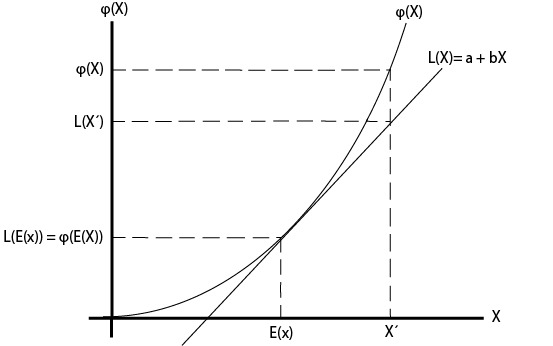
\includegraphics[scale=0.5]{img/Intuicion_Jensen.jpeg}
    \caption{Intuición geométrica de la desigualdad de Jensen }
    \label{fig:intuicion_jensen}
\end{figure}

Volviendo a lo anterior, utilizando las expresiones en \eqref{eq:total_expectation} y \eqref{eq:jensen_var}, podemos demostrar el teorema anterior.

 \begin{proof}[Demostración de Teorema \ref{teo:rao-blackwell}]
 	La varianza del estimador $\phi^\star$ está dada por 
 	\begin{alignat*}{2}
 		\Et{(\phi^\star-\theta)^2} &= \Et{(\Et{\phi|T}-\theta)^2} \quad\quad\quad &&\text{def.}\\
 								&= \Et{(\Et{\phi-\theta|T})^2}&& \text{linealidad}\\
 								&\leq \Et{\Et{(\phi-\theta)^2|T}}&& \text{Jensen}\\
 								&= \Et{(\phi-\theta)^2} &&\text{ley esperanzas totales}
 	\end{alignat*}
Donde las esperanzas exteriores son con respecto a $T$ y las interiores con respecto a $X$ (o equivalentemente a $\phi$).  Observemos además que la desigualdad anterior viene de la expresión en la ecuación \eqref{eq:jensen_var}, por lo que la igualdad es obtenida si $\V{\phi-\theta|T} = 0$, es decir, la VA $\phi-\theta$ tiene que ser constante para cada valor de $T$, es decir, $\phi$ es función de $T$. Intuitivamente podemos entender esto como que si el estadístico ya fue considerado en el estimador, entonces conocer el valor del estadístico no reporta información adicional. 
 \end{proof}

\begin{remark}
	Notemos que si el estimador $\phi$ es insesgado, su \textit{Rao-Blackwellización} $\phi^*$ también lo es, en efecto
	\begin{equation}
		\Et{\phi^*} = \Et{\Et{\phi|T}} = \Et{\phi} = \theta,
	\end{equation}
	donde la segunda igualdad está dada por la ley de esperanzas totales y la tercera por el supuesto de que $\phi$ es insesgado.
\end{remark}

\section{Varianza uniformemente mínima}

Observemos que, en base al riesgo cuadrático definido en la ecuación \eqref{eq:riesgo_cuad}, si un estimador es insesgado (Definición \ref{def:estimador_insesgado}) entonces su riesgo cuadrático es únicamente su varianza. Esto motiva la siguiente definición de optimalidad para estimadores insesgados. 

 \begin{definition}[Estimador insesgado de varianza uniformemente mínima]
  	El estimador $\phi=\phi(X)$ de $\theta$ es un estimador insesgado de varianza uniformemente mínima (EIVUM) si es insesgado y además si $\forall \phi':\cX\rightarrow \Theta$ estimador insesgado se tiene
  	\begin{equation}
  		\Vt{\phi}\leq\Vt{\phi'}, \forall \theta\in\Theta.
  	\end{equation}
  	Es decir, el EIVUM es el estimador insesgado que tiene menor varianza de todos los estimadores insesgados (y puede no ser único).
  \end{definition} 

\begin{example}
	Consideremos $X=(X_1,\ldots,X_n)\sim\ber{\theta}$ y los siguientes estimadores de $\theta$
	\begin{itemize}
		\item $\phi_1(X) = X_1$
		\item $\phi_2(X) = \frac{1}{2}(X_1+X_2)$
		\item $\phi_3(X) = \frac{1}{n}\sum_{i=1}^n X_i$
	\end{itemize}
	Observemos que todos estos estimadores son insesgados, pues como $\forall i, \Et{X_i} = \theta$, entonces 
	\begin{equation}
		\Et{\phi_1(X)} = \Et{\phi_2(X)} = \Et{\phi_3(X)} = \theta.
	\end{equation}
	Veamos ahora que la varianza de $\phi_3(X)$ está dada por
	\begin{equation}
		\Vt{\phi_3(X)} = \Vt{\frac{1}{n}\sum_{i=1}^n X_i} = \frac{1}{n^2}\sum_{i=1}^n \Vt{X_i} = \frac{\theta(1-\theta)}{n}
	\end{equation}
	pues $\Vt{X_i} = \Et{(\theta - X_i)^2} = \Et{X_i^2} - \theta^2 = (0^2 \cdot (1-\theta) + 1^2 \cdot \theta) - \theta^2 = \theta(1-\theta)$. Consecuentemente, la varianza de los estimadores considerados decae como la inversa del número de muestras $1/n$.
\end{example}

Con las definiciones anteriores, podemos mencionar el siguiente teorema, el cual conecta la noción de estadístico completo con la de EIVUM. 

\begin{theorem}[Teorema de Lehmann-Scheffé]
	Sea $X$ una VA con distribución paramétrica $\familiaparametrica$ y $T$ un estadístico suficiente y completo para $\theta$. Si el estimador $\phi = \phi(T)$ de $\theta$ es insesgado, entonces $\phi$ es el único EIVUM. 
 \end{theorem} 
 
 Es decir, el Teorema de Lehmann-Scheffé nos permite verificar que un estimador es el (único) EIVUM, si éste es insesgado y es función de un estadístico suficiente y completo. 
    

 \begin{proof}
 	Veamos en primer lugar que es posible construir un estimador en función del estadístico suficiente $\phi(T)$ que tiene menor o igual varianza que un estimador arbitrario $\phi'(X)$. En efecto, el Teorema de Rao-Blackwell establece que el estimador 
 	\begin{equation}
 		\phi(T) = \Et{\phi'(X)|T},
 	\end{equation}
 	tiene efectivamente menor (o igual) varianza que $\phi'(X)$.\\

 	Ahora veamos que solo existe un único estimador insesgado que es función del estadístico completo $T$. Asumiendo que existiesen dos estimadores insesgados de $\theta$ que son funciones de $T$, denotados $\phi_1(T),\phi_2(T)$, entonces, $\Et{\phi_1(T)-\phi_2(T)}=0$, es decir, $\phi(T) = \phi_1(T)-\phi_2(T)$ es un estimado insesgado de 0. Luego, como $T$ es completo, entonces, $\phi(T)=0$ es identicamente nulo, lo cual implica que  $\phi_1(T) = \phi_2(T)$ c.s.-$P_\theta$.\\

 	Hemos probado que (i) para un estimador arbitrario, se puede construir un estimador que es función de $T$ el cual tiene menor o igual varianza que el estimador original y, (ii) el estimador insesgado $\phi(T)$ es único. Consecuentemente, $\phi(T)$ es el único EIVUM.
 \end{proof}

El Teorema de Lehmann-Scheffé da una receta para encontrar el EIVUM: simplemente es necesario encontrar un estadístico completo y construir un estimador insesgado en base a éste, esto garantiza que el estimador construido es el \textbf{único} EIVUM.
\begin{example}[EIVUM para Bernoulli]
	Recordemos que en el Ejemplo \ref{eq:est_completo_bernoulli} vimos que el estadístico $T=\sum_{i=1}^nX_i$ es completo para $X\sim\ber{\theta}$. Como el estimador de $\theta$ dado por $\phi(T) = T/n$ es insesgado, 
\begin{equation}
	\Et{\phi(T)} = \Et{T/n} = \sum_{i=1}^n \Et{X_i} /n = \theta,
\end{equation}
entonces $\phi(T) = T/n$ es el EIVUM para $\theta$ en $\ber{\theta}$ y es único.	
\end{example}

\begin{remark}
Lectura personal: Estadístico auxiliar (ancilliary) y teoremas de Basur y de Bahadur. 
\end{remark}
\section{Ejercicios}

\begin{enumerate}
    \item Se quiere estudiar el comportamiento de un vector bidimensional que tiene sus dos componentes ortogonales, independientes y que siguen una distribución normal. Al realizar las mediciones respectivas de cada componente, se obtiene una Muestra Aleatoria Simple (MAS, cada dato es generado desde una misma distribución y son independientes entre sí (iid)) $U=(U_1,...,U_n)$ de $n$ observaciones con $U_n\sim\mathcal{N}(0,\sigma^2)$  y una MAS $W=(W_1,...,W_n)$  de $n$ observaciones con $W_n\sim\mathcal{N}(0,\sigma^2)$. En específico, se busca estudiar el comportamiento de los módulos de los vectores obtenidos. Se obtiene una nueva MAS $X=(X_1,...,X_n)$ dada por:

\[X_i = \sqrt{U_i^2 - W_i^2}\]

\begin{enumerate}
    \item [i.] Encuentre la función de densidad de $X_1$\\
\end{enumerate}

\item Estudiaremos la varianza $\sigma^2$ de una Muestra Aleatoria Simple (MAS) $X=(X_1,...,X_n)$ donde $X_i\sim\mathcal{N}(\mu, \sigma^2)$, $\forall i =1,...,n$. Se considera que $\mu$ y $\sigma$ son parámetros desconocidos. 

Considere el siguiente estimador de la varianza dado por:

\[S^2 := \frac{1}{n-1}\sum\limits_{i=1}^{n}(\overline{X}_n-X_i)^2\]
donde $\overline{X}_n$ denota al promedio de $X_1,..., X_n$, es decir  $\overline{X}_n = \sum\limits_{i=1}^{n}X_i$. 
\begin{enumerate}
    \item [i.] Demuestre que $\mathbb{E}(S^2) = \sigma^2$ 
    \item [ii.] Calcule la varianza de $S^2$, para esto encontraremos primero la distribución de $\frac{n-1}{\sigma^2}S^2$, siga los siguientes pasos:
    \begin{enumerate}
        \item [ii.a.] Desarrolle la expresión $W=\sum\limits_{i=1}^{n}\frac{(X_i-\mu)^2}{\sigma^2}$ para llegar a:
        \[W = \frac{(n-1)}{\sigma^2}S^2  + \frac{n(\overline{X}_n-\mu)^2}{\sigma^2} \]
        \item [ii.b.] Encuentre las distribuciones asociadas a W y a $\frac{n(\overline{X}_n-\mu)^2}{\sigma^2} $
        \item [ii.c.] Aplique la función generadora de momentos en ambos lados de la ecuación. Para esto, asuma que $S^2$ es independiente de $\overline{X}_n$.
        \item [ii.d.] Encuentre la distribución de $\frac{n-1}{\sigma^2}S^2$
        \item [ii.e.] Calcule $\mathbb{V}(S^2)$
    \end{enumerate}
    \item [iii.] (Ejercicio) Calcule la varianza de $S^2$ desarrollando \textit{a mano} (Muy largo). 
\end{enumerate}


Ahora se considera otro estimador de la varianza dado por:

\[\hat{\sigma}^2 := \frac{1}{n}\sum\limits_{i=1}^{n}(\overline{X}_n - X_i)^2    \]

\begin{enumerate}
    \item [iv.] Muestre que $\hat{\sigma}^2$ cumple que $\mathbb{E}(\hat{\sigma}^2) \neq \sigma^2$ 
    \item [v.] Muestre que $\hat{\sigma}^2$ cumple que $\lim\limits_{n\rightarrow \infty} \mathbb{E}(\hat{\sigma}^2) = \sigma^2$
\end{enumerate}

\begin{enumerate}
    \item [vi.] Calcule $ECM_{\sigma^2}(S^2)$
    \item [vii.] Calcule $ECM_{\sigma^2}(\hat{\sigma}^2) $
    \item [viii.] Verifique que $ECM_{\sigma^2}(\hat{\sigma}^2) < ECM_{\sigma^2}(S^2)$
\end{enumerate}
\end{enumerate}

\chapter{Enfoque bayesiano}

En esta sección complementaremos el enfoque visto hasta ahora en cuanto a la incorporación de un modelo para la incertidumbre asociada al parámetro $\theta$. En el paradigma bayesiano, consideraremos que el parámetro es una variable aleatoria, es decir, $\Theta$, la cual para una realización particular tomar el valor $\Theta = \theta$. Esto nos permite información \emph{a priori} sobre la estimación a realizar, lo que permite, en muchos casos, ayudar a la inferencia. Una diferencia conceptual entre ambos enfoques, es que la estadística frecuentista evita la subjetividad, mientras que la estadística bayesiana se basa en la convicción del(a) investigador(a), para emitir juicios sobre una hipótesis.

En este capítulo, se estudiará la estadística bayesiana y se introducirán los mismos conceptos vistos anteriormente desde el punto de vista bayesiano.




\section{Contexto y definiciones principales}

\begin{definition}[Distribución a priori]
La información, sesgos y cualquier otra característica conocida de $\Theta$ codificadas mediante la propia ley de probabilidad de esta VA, la cual tiene densidad $p(\theta)$, nos referimos a esta como la \emph{densidad a priori} o simplemente \emph{prior}.
\end{definition}

Con esta definición, podemos ver que la densidad conjunta de las VAs $X,\Theta$ pueden ser expresadas combinando la densidad a priori con el modelo visto en las secciones anteriores, es decir, 
\begin{equation}
    p(x,\theta) = p(x|\theta)p(\theta)
    \label{eq:joint_bayes}
\end{equation}
donde hemos escrito $p(x|\theta)$ en vez de $p_\theta(x)$ para hacer explícito que ahora consideramos el parámetro como una variable aleatoria. 

Adicionalmente, con la distribución conjunta en la ecuación \eqref{eq:joint_bayes}, podemos definir:

\begin{definition}[Distribución marginal]
La distribución de $X$, obtenida mediante la desintegración de parámetro $\Theta$ del par $(X,\Theta)$, es decir 
\begin{equation}
    p(x) = \int_\Omega p(x|\theta)p(\theta)\d\theta
\end{equation}
es conocida como distribución marginal de $X$.
\end{definition}

Consideremos ahora que tenemos un conjunto de observaciones denotado por $\mathcal{D}$, de un modelo estadístico con parámetro $\Theta$, entonces podemos definir

\begin{definition}[Función de verosimilitud]
La densidad de probabilidad evaluada en un conjunto de observaciones $\cD$ como función del valor del parámetro $\Theta$, es decir 
\begin{align}
    L: \Omega &\rightarrow \R\\
    \theta&\mapsto l(\theta) = L_\cD(\theta) = p(\cD|\theta),
\end{align}
recibe el nombre de función de verosimilitud, o en inglés, \emph{likelihood}. 
\label{función_verosimilitud}
\end{definition}
\begin{remark}
La función de verosimilitud no es una densidad de probabilidad, es decir, no es cierto que
\begin{equation}
    \int_\Omega L(\theta)\d\theta = 1
\end{equation}
\end{remark}

\begin{remark}
Dado que la función función de verosimilitud usualmente adquiere una forma exponencial (como por ejemplo en el caso de la familia exponencial), hay ocasiones en donde es conveniente usar la \emph{log-verosmilitud}, esto es, 
\begin{equation}
l(\theta)=\log L(\theta)=\log p(\cD|\theta).
\end{equation}
Esta formulación será particularmente útil cuando queramos optimizar la verosimilitud. 
\end{remark}

\begin{remark}
En general (pero no siempre) asumimos observaciones $\cD = {X_1,\ldots,X_n}$, $X_i\sim p(x|\theta)$, que son i.i.d. En cuyo caso, la verosimilitud factoriza de la forma $L_\cD(\theta) = \prod_{i=1}^n L_{X_i}(\theta)$, con lo cual la log-verosimilitud toma la forma: 
\begin{equation}
l_\cD(\theta) = \sum_{i=1}^nl_{X_i}(\theta)
\end{equation}
\end{remark}

\begin{example}
Considere los datos $\cD = \{x_1,...,x_n\}$, donde $x_i$ es la observación de una VA $X_i\sim \mathcal{N}(\mu,\sigma^2)$ iid con $\sigma^2$ conocido. La función  de verosimilitud de $\mu$ está dada por:

\begin{align}
L(\mu)=p(\cD|\mu)&=\prod_{i=1}^{n} \frac{1}{\sqrt{2 \pi \sigma^{2}}} 
\exp\left(\frac{-1}{2\sigma^{2}}(x_i-\mu)^{2}\right)\nonumber\\
&= \left(\frac{1}{\sqrt{2 \pi \sigma^{2}}}\right)^{n} \exp\left(\frac{-1}{2 \sigma^{2}} \sum_{i=1}^{n} (x_i - \mu )^{2}\right).
\end{align}

Luego, la log-verosimilitud está dada por:
\begin{equation}
    l(\mu)= \log L(\mu) = -\frac{n}{2} \log(2 \pi \sigma^{2}) + \frac{-1}{2\sigma^{2}} \sum_{i=1}^{n} (x_i - \mu )^{2}.
\end{equation}

\end{example}

Ahora estamos en condiciones de definir el elemento central de la inferencia bayesiana, sobre el cual todo el proceso de inferencia toma lugar. 

\begin{definition}[Distribución posterior]
\label{dist_posterior}
Dado el conjunto de observación $\cD$ la distribución \emph{posterior} del parámetro, es decir, considerando la inforamción reportada por los datos $\cD$, está dada por el teorema de Bayes mediante
\begin{align}
    p(\theta|\cD) = \frac{p(\cD)|\theta)p(\theta)}{p(\cD)}  \propto p(\mathcal{D}|\theta) p(\theta) \label{eq:posterior_def}
\end{align}

donde: 
\begin{itemize}
    \item $p(\theta)$ es el prior del parámetro.
    \item $p(\theta|\mathcal{D})$ es la posterior del parámetro. 
    \item $p(\mathcal{D}|\theta)$ es la verosimilitud
    \item $p(\mathcal{D}) = \int\Omega p(\mathcal{D}|\theta)p(\theta)\d \theta $ es la densidad marginal de los datos 
\end{itemize}
\end{definition}

La \emph{transición} de prior a posterior puede ser interpretada como el proceso de incorporar la evidencia de los datos (a través de la función de verosimilitud) para reducir la incertidumbre con respecto del valor del parámetro $\Theta$. De la ecuación \eqref{eq:posterior_def} podemos ver que este proceso, a veces referido como \emph{actualización bayesiana}, equivale a multiplicar por la verosimilitud, para luego normalizar, garantizando que $p(\theta|\cD)$ es en efecto una densidad de probabilidad. 

\begin{remark}
El símbolo $\propto$ en la ecuación \eqref{eq:posterior_def} es usado para indicar que el lado izquierdo es igual al lado derecho salvo una constante de proporcionalidad que depende de $\mathcal{D}$ y no de $\theta$. Con esto, cuando estemos calculando la posterior, solo nos enfocaremos en \emph{una versión proporcional}, pues luego la densidad posterior se puede encontrar mediante la normalización de esta última.
\end{remark}

\begin{example}[Posterior modelo Bernoulli]
\label{ej_post_bernoulli_1}
Sea $\theta$ la probabilidad de obtener cara al lanzar una moneda, y sean $X_1,..X_n$ $n$ resultados obtenidos al lanzar la moneda. Si no sabemos nada de $\theta$ antes del experimento, hace sentido tomar su prior como una distribución que de igual probabilidad a todo espacio de parámetros, es decir: $\theta \sim Unif(0,1)$. Notemos que el prior encapsula la infromación que tenemos antes del experimento. Modelamos $X_1,..X_n \sim Bernoulli(\theta)$. Entonces: 
$$
p(X_1,..X_n|\theta)=\prod_{i=1}^{n} \theta^{X_i} (1-\theta)^{1-X_i} = 
\theta^{\sum_{i=1}^{n} X_i} (1-\theta)^{n-\sum_{i=1}^{n}X_i}
$$
Notemos que en este caso, podemos calcular la distribución $p(X_1,..,X_n)$:
$$
p(X_1,..,X_n)=\int_{0}^{1} \theta^{\sum_{i=1}^{n} X_i} (1-\theta)^{n-\sum_{i=1}^{n}X_i} d\theta = B\left(\sum_{i=1}^{n} X_i +1 , n- \sum_{i=1}^{n} X_i +1 \right),
$$
donde $B(x,y)$ es la función beta:
$$
B(x,y)=\dfrac{\Gamma(x)\Gamma(y)}{\Gamma(x+y)}.
$$
Sea $s= \sum_{i=1}^{n}X_i$. Entonces la distribución a posteriori será:

$$
p(\theta|X_1,..X_n)= \dfrac{p(X_1,..X_n|\theta)}{p(X_1,..,X_n)} = \dfrac{1}{B(s+1,n-s+1)} \theta^{s} (1-\theta)^{n-s}.
$$

\end{example} 

Usualmente, es experimentos reales, los datos  $x_1,...,x_n$ son recibidos de forma secuencial, es decir, \emph{en línea}. De esta forma, es relevante notar que en primer lugar se observa $x_1$ primero, luego $x_2$, y así sucesivamente. \\

Consecuentemente, si se asume el prior para el parámetro $\theta$ dado por $p(\theta)$, es posible hacer la actualización bayesiana \emph{en línea} (o de forma adaptativa o continual), lo cual implica una corrección del modelo cada vez que se observan más datos. \\
Luego de observar $x_1$, la posterior $p(\theta|x_1)$ puede ser calculada como: 
$$
p(\theta|x_1) \propto p(x_1|\theta) p(\theta).
$$

Luego, al observar $x_2$, usamos el hecho que $X_1$ y $X_2$ son condicionalmente independientes dado $\theta$ y obtenemos: 
$$
p(\theta | x_1,x_2) \propto 
p(x_2|\theta) p(\theta|x_1) \propto p(x_1 |\theta) p(x_2|\theta) p(\theta) . 
$$
Con lo que para el caso general tenemos que 
$$
p(\theta | x_1,..x_n) \propto p(x_n|\theta) p(\theta|x_1,..x_{n-1}) \propto p(\theta) \prod_{i=1}^n p(\theta | x_i).
$$

\begin{remark}
Cuando las observaciones $\cD$ son condicionalmente independientes dado el parámetro $\theta$, entonces, la posterior $p(\theta|\cD)$ factoriza en las verosimilitudes de cada uno de los datos. 
\end{remark}

\begin{remark}
En la actualización bayesiana en línea, la posterior de la etapa $n$ sirve de prior de la etapa $n+1$.
\end{remark}


\section{Priors Conjugados}

La actualización bayesiana puede resultar en una posterior solo conocida de forma proporcional (cuando no es posible calcular la distribución marginal $p(x)$) o bien en una distribución que no pertenece a una familia conocida. Una herramienta que asegurar el cálculo de las distribuciones posteriores (incluyendo la constante de normalización) y que esta adopta una forma conocida es a través del uso de \textbf{priors conjugados}.
\begin{definition}

Sea un modelo con verosimilitud $p(x|\theta)$ y un prior sobre $\theta$ con densidad $p(\theta)$. Decimos que $p(\theta)$ es conjugado con la verosimiltud $p(x|\theta)$ si la posterior 
\begin{equation}
	p(\theta|x) = \frac{p(x|\theta)p(\theta)}{p(x)}
\end{equation}
pertenece a la\textit{misma familia} que el prior $p(\theta)$. Donde pertenecer a la misma familia quiere decir que ambas tienen una densidad de probabilidad definida por la misma forma funcional, e.g., $f_\lambda(\theta)$ pero con distintos valores para el \textit{parámetro} $\lambda$, el cual es un \textit{hiperparámetro} del modelo.
\end{definition}


\begin{example}[continuación de Ejemplo \ref{ej_post_bernoulli_1}]
\label{ej_post_bernoulli_2}
Tarea: Verifique si el Ejemplo \ref{ej_post_bernoulli_1} es en efecto uno de prior conjugado. 
\end{example}

\begin{example}[Distribución Multinomial]
Consideremos una variable aleatoria multinomial $X\sim\mul{n,\theta}$ donde $\theta$ pertenece al simplex 
\begin{equation}
	\label{eq:simplex}
  \{\theta\in[0,1]^k:\theta_1 + \cdots + \theta_k = 1 \}.
 \end{equation} 
 La distribución multinomial genera vectores $X\in\N^k$ cuya $i-$ésima componente modela la cantidad de veces que ocurre el evento $i$ dentro de $k$ eventos en $n$ intentos. Por ejemplo, si lanzamos un dado balanceado 100 veces, el vector que contiene el conteo de veces que obtenemos cada cara puede modelarse como 
 \begin{equation}
  	\theta_\text{dado} \sim \mul{100,\left[\tfrac{1}{6},\tfrac{1}{6},\tfrac{1}{6},\tfrac{1}{6},\tfrac{1}{6},\tfrac{1}{6}\right]}.
  \end{equation} 
Denotando $X=[x_1,\ldots,x_n]$, observemos que una muestra multinomial $X\sim\mul{n,\theta}$ cumple con 
\begin{equation}
	\{x_i\}_{i=1}^k \subset \{0,1,\ldots,n\},\quad  \sum_{i=1}^kx_i = n.
\end{equation}

Finalmente, la distribución Multinomial está dada por 
\begin{equation}
 	\mul{X;n,\theta} = \frac{n!}{x_1!\cdots x_k!} \theta_1^{x_1}\cdots\theta_k^{x_k},
 \end{equation} 
 y es la generalización de las distribuciones: 
\begin{itemize}
	\item Bernoulli cuando $k=2$ y $n=1$; pues $\ber{X;\theta} = \theta^{x} (1-\theta)^{1-x}$
	\item Categórica (o \emph{multinoulli}): cuando $n=1$; pues $\cat{X;\theta} = \theta_1^{x_1}\cdots\theta_k^{x_k}$
	\item Binomial: cuando $k=2$; pues $\bin{X;n,\theta} = \binom{n}{x} \theta^{x}(1-\theta)^{n-x}$
\end{itemize}
\end{example}

Observemos que el parámetro $\theta$ en la distribución multinomial (y las otras tres) es precisamente una distribución de probabilidad (discreta). Es decir, el construir un prior $p(\theta)$ implica definir una distribución sobre distribuciones discretas.  


\begin{definition}[Distribución de Dirichlet]
Consideremos la  distribución de Dirichlet
\begin{equation}
	\theta \sim \dir{\theta|\alpha} = \frac{1}{B(\alpha)} \prod_{i=1}^k \theta_i^{\alpha_i-1},
\end{equation}
donde $\alpha = (\alpha_1,\ldots,\alpha_k)$ es el parámetro de concentración y la constante de normalización está dada por $B(\alpha)=\prod_{i=1}^k\Gamma(\alpha_i)/\Gamma(\sum_{i=1}^k\alpha_i)$. El soporte de esta distribución es el simplex presentado en la ecuación \eqref{eq:simplex}.
\end{definition}


En el caso $k=3$, la distribución de Dirichlet puede ser graficada en el simplex de 2 dimensiones. La Figura \ref{fig:dist_Dirichlet} presenta tres gráficos para distintos valores del parámetro de concentración. 

\begin{figure}[H]

\includegraphics[width=0.3\textwidth]{img/dirichlet111.png}
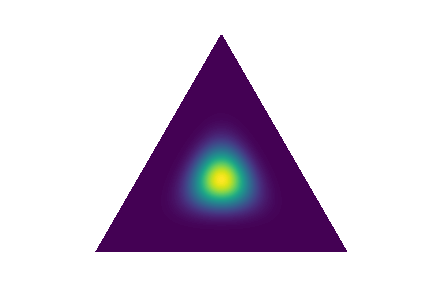
\includegraphics[width=0.3\textwidth]{img/dirichlet101010.png}
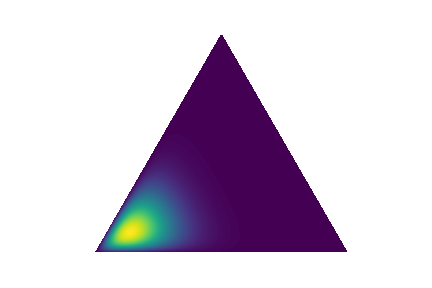
\includegraphics[width=0.3\textwidth]{img/dirichlet1022.png}
\caption{Distribuciones Dirichlet para $k=3$ con parámetros de concentración $\alpha$ (desde izquierda a derecha) dado por $[1,1,1]$, $[10,10,10]$ y $[10,2,2]$. }.
\label{fig:dist_Dirichlet}
\centering
\end{figure}


Veamos a continuación que la distribución de Dirichlet es conjugada al modelo Multinomial, y consecuentemente para Bernoulli, Categórica y Binomial. En efecto, si $\theta \sim \dir{\theta;\alpha}$ y $X\sim\mul{X;n,\theta}$, entonces

\begin{align}
	p(\theta|x) &= \frac{\mul{x;n,\theta}\dir{\theta;\alpha}}{p(x)}\nonumber\\
				&=  \frac{n!}{ x_1!\cdots x_k!p(x) B(\alpha)} \prod_{i=1}^k \theta_i^{x_i + \alpha_i-1}\nonumber\\
				&=  \frac{1}{B(\alpha')} \prod_{i=1}^k \theta_i^{\alpha'_i-1}
				\label{eq:dirichlet_post}
\end{align}
donde $\alpha' = (\alpha'_1,\ldots,\alpha'_k) = (\alpha'_1 + x_1,\ldots,\alpha'_k+ x_k)$ es el nuevo parámetro de concentración.

\begin{example}
	Consideremos $\alpha = [1,2,3,4,5]$ y generemos una muestra de $\theta\sim\dir{\theta|\alpha}$. El siguiente código genera, grafica e imprime esta muestra. 
	\begin{lstlisting}[language=Python]
	import numpy as np
	alpha = np.array([1,2,3,4,5]) 
	theta = np.random.dirichlet(alpha)
	plt.bar(np.arange(5)+1, theta);
	print(f'theta = {theta}')
\end{lstlisting}
En nuestro caso, obtuvimos los parámetros $ \theta = [0.034, 0.171, 0.286, 0.185, 0.324]$.

 Ahora, usaremos un prior Dirichlet sobre $\theta$ con $\alpha_p = [1,1,1,1,1]$ para calcular la posterior de acuerdo a la ecuación \eqref{eq:dirichlet_post}. La Figura \ref{fig:post_Dirichlet} muestra 50 muestras de la distribución posterior para distintas cantidades de observaciones entre 0 y  $ 10^5$. 

\begin{figure}[H]
\centering
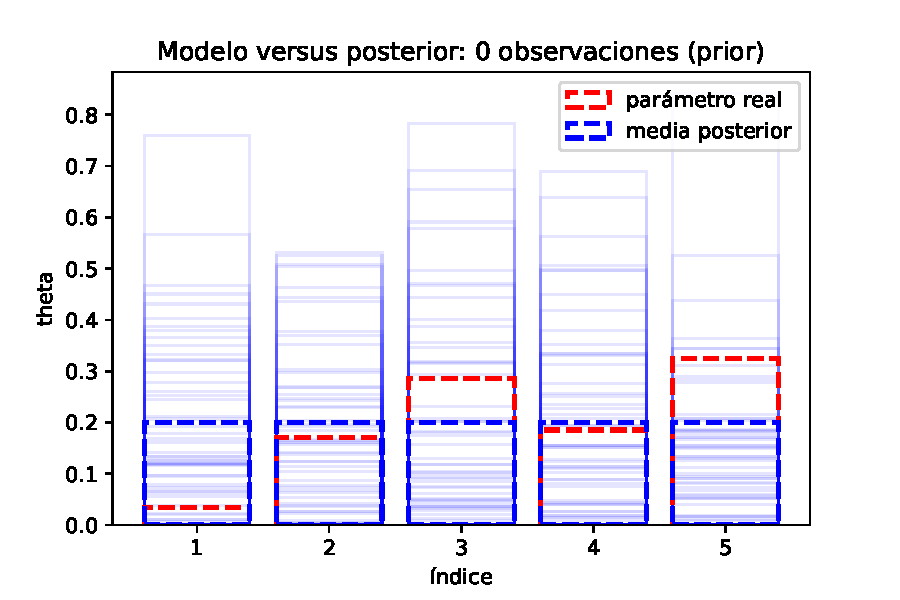
\includegraphics[width=0.3\textwidth]{img/post_dirichlet_0.pdf}
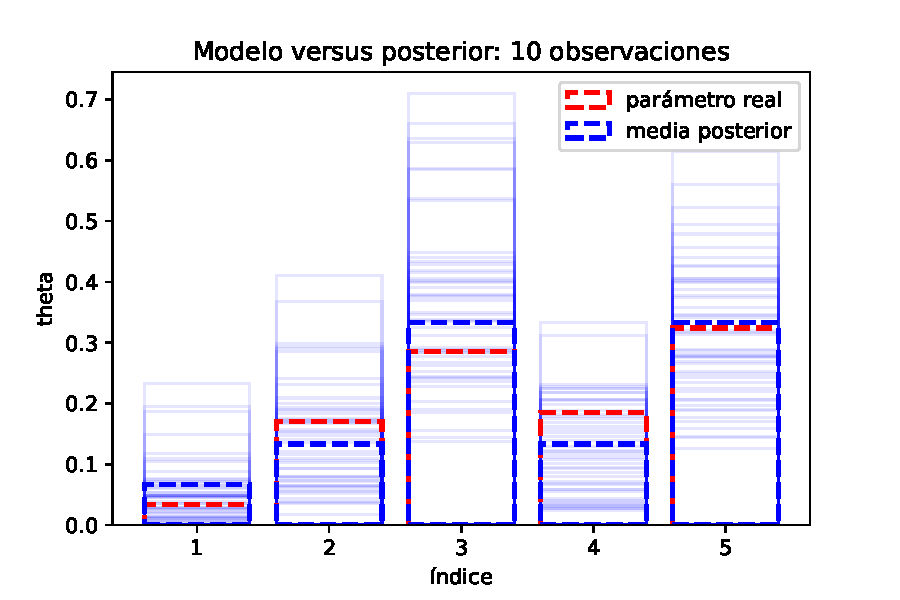
\includegraphics[width=0.3\textwidth]{img/post_dirichlet_10.pdf}
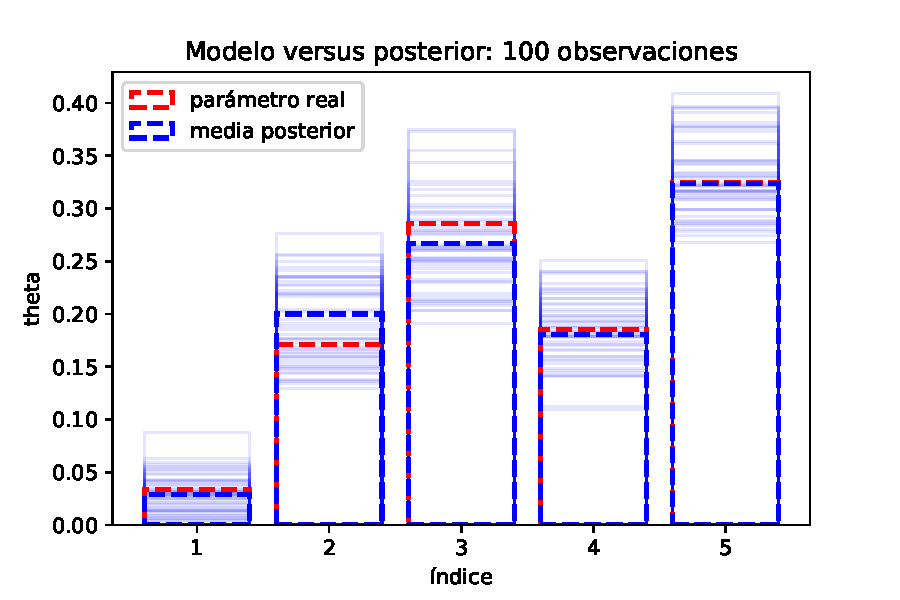
\includegraphics[width=0.3\textwidth]{img/post_dirichlet_100.pdf}\\
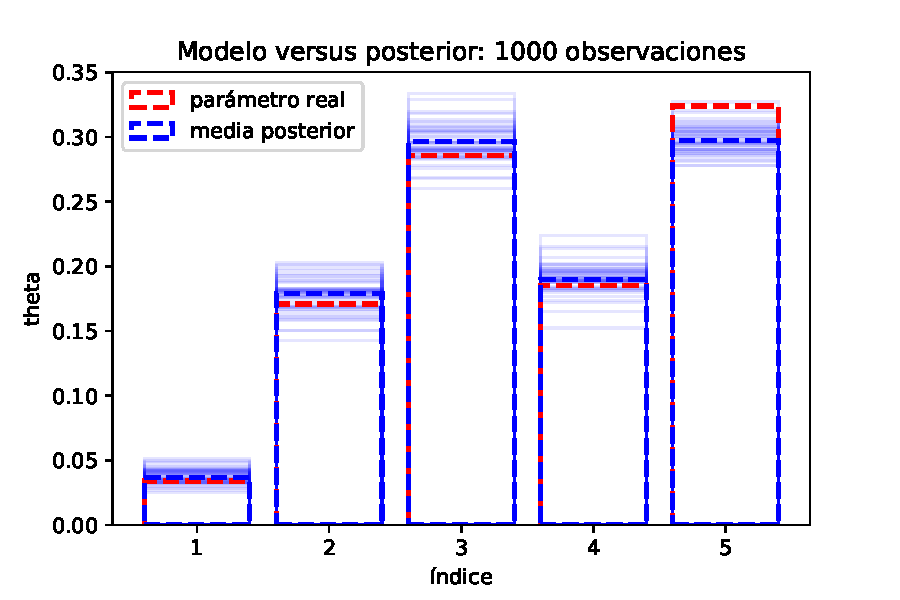
\includegraphics[width=0.3\textwidth]{img/post_dirichlet_1000.pdf}
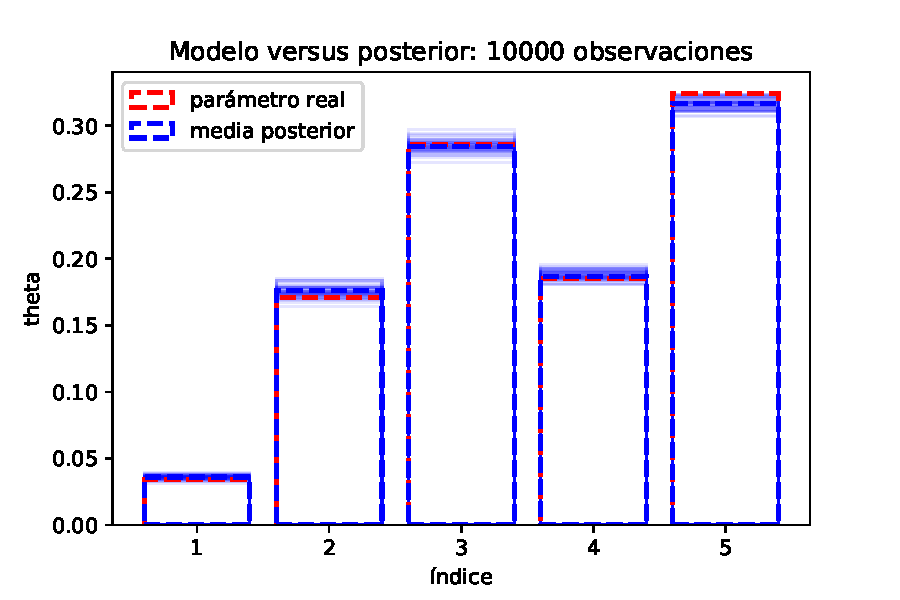
\includegraphics[width=0.3\textwidth]{img/post_dirichlet_10000.pdf}
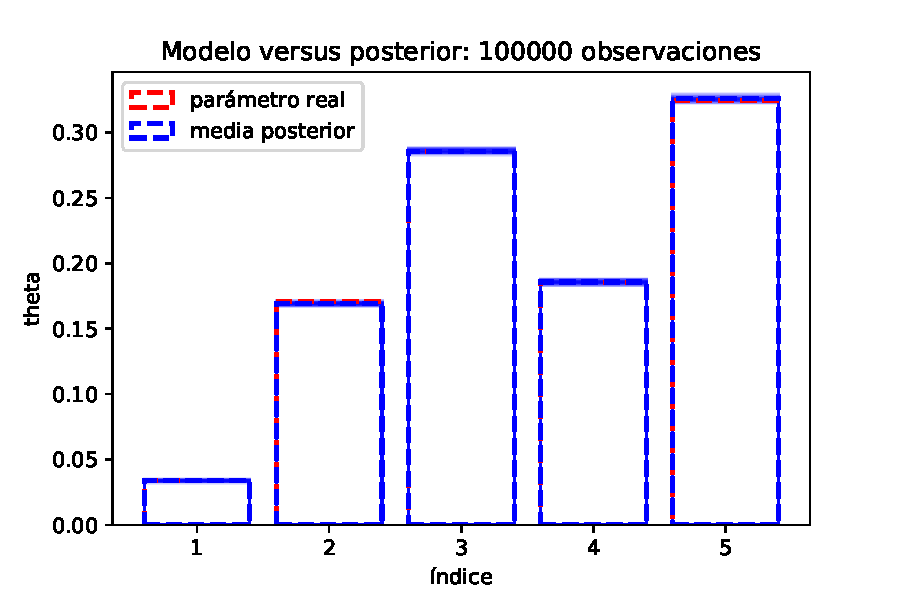
\includegraphics[width=0.3\textwidth]{img/post_dirichlet_100000.pdf}
\caption{Concentración de la distribución posterior en torno al parámetro real para un modelo $X\sim\mul{\theta}$ y una distribución a priori Dirichlet $\theta\sim\dir{\alpha}$. Se considera desde 0 hasta $10^5$ observaciones y cada gráfico (desde izquierda-arriba hasta derecha-abajo) muestra el parámetro real (linea roja quebrada), la media posterior (línea azul quebrada) y 50 muestras de la posterior (azul claro). Observe cómo la distribución a priori (línea azul quebrada en la primera figura) pierde importancia a medida que el número de observaciones aumenta.}
\label{fig:post_Dirichlet}
\end{figure}
\end{example}


\begin{example} \textbf{Modelo gaussiano ($\sigma^2$ conocido).} Consideremos el prior sobre la media $p(\mu) = \cN(\mu_0,\sigma_0^2)$, con lo que la posterior está dada por  
 \begin{align}
 	p(\mu|\mathcal{D}) &\propto \prod_{i=1}^n \frac{1}{\sqrt{2\pi\sigma^2}}\exp\left(-\frac{1}{2\sigma^2}(x_i-\mu)^2\right) \frac{1}{\sqrt{2\pi\sigma_0^2}}\exp\left(-\frac{1}{2\sigma_0^2}(\mu-\mu_0)^2\right)\label{eq:post_normal_mu_1}\\
 	&\propto \exp\left(-\frac{1}{2\sigma^2}\sum_{i=1}^n(x_i-\mu)^2-\frac{1}{2\sigma_0^2}(\mu-\mu_0)^2\right),\label{eq:post_normal_mu_2}
 \end{align} 
 donde la proporcionalidad viene de ignorar la constante $p(\mathcal{D})$ en la primera línea e ignorar todas las contantes que no dependen de $\mu$ en la segunda línea. Recordemos que estas constantes para $\mu$ incluyen a la varianza de $x$, $\sigma^2$, por lo que ignorar esta cantidad es solo posible debido a que estamos considerando el caso en que $\sigma^2$ es conocido. Completando la forma cuadrática para $\mu$ dentro de la exponencial en la ec.~\eqref{eq:post_normal_mu_2}, obtenemos
 \begin{equation}
 	p(\mu|\mathcal{D}) \propto \exp\left(-\frac{1}{2\sigma_n^2}(\mu - \mu_n)^2\right),\label{eq:post_normal_mu_3}
 \end{equation} 
 donde (ya definiremos $\mu_n$ y $\sigma_n^2$ en breve) como $p(\mu|\mathcal{D})$ debe integrar uno, la única densidad de probabilidad proporcional al lado derecho de la ecuación anterior es la Gaussiana de media $\mu_n$ y varianza $\sigma_n^2$. Es decir, la constante de proporcionalidad necesaria para la igualdad en la expresión anterior es
 \begin{equation}
     \int_\R\exp\left(-\frac{1}{2\sigma_n^2}(\mu - \mu_n)^2\right)\d\mu = (2\pi\sigma_n^2)^{n/2}.
 \end{equation} Consecuentemente, confirmamos que el prior elegido era efectivamente conjugado con la verosimilitud gaussiana, con lo que la posterior está dada por la siguiente densidad (gaussiana):
  \begin{equation}
 	p(\mu|\mathcal{D}) = \cN(\mu;\mu_n,\sigma_n^2) = \frac{1}{(2\pi\sigma_n^2)^{N/2}}\exp\left(-\frac{1}{2\sigma_n^2}(\mu - \mu_n)^2\right),\label{eq:post_normal_mu_4}
 \end{equation} 
 donde la media y la varianza están dadas respectivamente  por 
 \begin{align}
 	\mu_n &= \frac{1}{\tfrac{1}{\sigma_0^2} + \tfrac{n}{\sigma^2}} \left(\frac{1}{\sigma_0^2}\mu_0 + \frac{n}{\sigma^2}\bar{x} \right), \quad \text{donde } \bar{x} = \frac{1}{n}\sum_{i=1}^n x_i\label{eq:post_Gm}\\
 	\sigma_n &= \left(\frac{1}{\sigma_0^2} + \frac{n}{\sigma^2}\right)^{-1}.\label{eq:post_Gv}
 \end{align}
\end{example}
\begin{remark}
	La actualización bayesiana transforma los parámetros del prior de  $\mu$ desde  $\mu_0$ y $\sigma_0^2$ hacia $\mu_n$ y $\sigma_n^2$ en las ecs.~\eqref{eq:post_Gm} y \eqref{eq:post_Gv} respectivamente. Notemos que los  parámetros de la posterior son combinaciones (interpretables por lo demás) entre los parámetros del prior y los datos, en efecto, la $\mu_n$ es el promedio ponderado entre  $\mu_0$ (que es nuestro candidato para $\mu$ antes de ver datos) con factor $\sigma_0^{-2}$ y el promedio de los datos $\bar{x}$ con factor $(\sigma^{2}/n)^{-1}$, que a su vez es el estimador de máxima verosimilitud. Es importante también notar que  estos  factores son las varianzas inversas---i.e., precisión---de $\mu_0$ y de $\bar{x}$. Finalmente, observemos que $\sigma_n$ es la \emph{suma paralela} de las varianzas, pues  si expresamos la ec.~\eqref{eq:post_Gv} en términos de \emph{precisiones}, vemos que la precisión inicial $\sigma_0^2$ aumenta un término $\sigma^2$ con cada dato que vemos; lo cual tiene sentido pues con más información es la precisión la que debe aumentar y no la incertidumbre (en este caso representada por la varianza).
\end{remark}
\begin{example} \textbf{Modelo gaussiano ($\mu$ conocido).} Ahora procedemos con el siguiente prior para la varianza, llamado Gamma-inverso:
 \begin{equation}
 	p(\sigma^2)= \text{inv-}\Gamma(\sigma^2;\alpha,\beta) = \frac{\beta^\alpha}{\Gamma(\alpha) (\sigma^2)^{\alpha+1}}\exp(-\beta/\sigma^2)
 \end{equation}
 esta densidad recibe dicho nombre pues es equivalente a modelar la precisión, definida como el recíproco de la varianza $1/\sigma^2$, mediante la distribución Gamma. Los hiperparámetros $\alpha$ y $\beta$ son conocidos como parámetros de forma y de tasa (o precisión) respectivamente. 

 Con este prior, la posterior de la varianza toma la forma:
 \begin{align}
 	p(\sigma^2|\mathcal{D}) &\propto \prod_{i=1}^N \frac{1}{\sqrt{2\pi\sigma^2}}\exp\left(-\frac{1}{2\sigma^2}(x_i-\mu)^2\right) \frac{\beta^\alpha}{\Gamma(\alpha) (\sigma^2)^{\alpha+1}}\exp(-\beta/\sigma^2)\\
 	&\propto  \frac{1}{(\sigma^2)^{N/2+\alpha+1}}\exp\left(-\frac{1}{\sigma^2}\left(\frac{1}{2}\sum_{i=1}^N(x_i-\mu)^2 +\beta\right) \right)\nonumber
 \end{align} 
 donde nuevamente la proporcionalidad ha sido mantenida debido a la remoción de las constantes. Esta última expresión es proporcional a una distribución Gamma inversa con hiperparámetros $\alpha$ y $\beta$ ajustados en base a los datos observados. 


\end{example}




Hay ocasiones en las que el conocimiento a priori sobre el parámetro no puede ser convenientemente expresado mediante una densidad de probabilidad pero sí una densidad que no necesariamente integra uno o incluso es (Lebesgue) integrable. Para reflejar esta idea, se usan priors impropios.

\begin{definition}[Prior impropia] Una distribución a priori impropia es una distribución que no es necesariamente de probabilidad (i.e., no integra 1), pero que de todas formas puede ser utilizada como distribución a priori en el contexto de inferencia bayesiana, pues la distribución posterior correspondiente si es una distribución de probabilidad apropiada. 
\end{definition}

\begin{remark} No es necesario usar la constante de normalización en las densidades a priori Gaussianas (o ninguna otra en realidad).
\end{remark}

\begin{remark} Veamos que un prior impropio puede incluso tener integral infinita, en el caso de la distribución normal $X\sim\cN(X;\mu,1)$,  $\mu\in\R$, podemos elegir $p(\mu)\propto1$ y escribir 
\begin{equation}
	p(\mu|x)\propto p(x|\mu)\cdot 1 = \cN(x;\mu,1) = \cN(\mu;x,1). 
\end{equation}
	
\end{remark}

Considerar distribuciones uniformes impropias como priors no informativas parece tener sentido, pues intuitivamente no estamos dando preferencia (mayor probabilidad a priori) a ningún valor del parámetro por sobre otro. Sin embargo, este procedimiento sufre de una desventaja conceptual.




\section{Estimación y predicción}

\subsection{Estimadores bayesianos}

Si bien ya hemos estudiado el rol del prior en la inferencia bayesiana, hasta ahora no lo hemos considerado en la construcción de estimadores. En particular, el EMV no incorpora conocimiento a priori del parámetro. Con el objetivo de incorporar este conocimiento a priori en el cálculo de estimadores puntales, consideramos que en el caso general, podemos considerar otros estimadores puntuales a través de una función de pérdida asociada a estimar el parámetro $\theta$ mediante el estimador $\hat\theta$ dada por $L(\theta,\hat\theta)$. Con esto podemos definir los conceptos de riesgo y estimador bayesiano.

\begin{definition}[Riesgo bayesiano]
Para una función de pérdida $L(\theta,\hat\theta)$ y un conjunto de observaciones $\cD$, el riesgo bayesiano es la esperanza posterior de dicha función de pérdida, es decir
\begin{equation}
    R(\hat\theta) = \int_\Omega L(\theta,\hat\theta)p(\theta|\cD)\d\theta.
\end{equation}
\end{definition}



\begin{definition}[Estimador bayesiano]
Dado un conjunto de datos $\cD$ y un riesgo bayesiano $R(\theta)$, un estimador bayesiano es uno que minimiza el riesgo bayesiano:
\begin{equation}
    \theta_\text{Bayes}(\cD) = \arg\min_{\Omega} R(\theta).
\end{equation}
donde es implícito que $R(\cdot)$ se define con $\cD$.
\end{definition}

A continuación, se definirán estimadores bayesianos  con distintas funciones de costo o de riesgo.


\begin{definition}[Bayes' Least-Squares (BLS)]
El  caso estándar es la función de pérdida cuadrática $L_2(\theta,\hat\theta) = (\theta-\hat\theta)^2$ la cual resulta en el estimador dado por la media posterior $\theta_\text{Bayes}(\cD) = \E{\theta|\cD}$
\end{definition}


\begin{definition}[Minimum absolute-error (MAE)]

De forma similar,la función de costo $L_1(\theta,\hat\theta) = |\theta-\hat\theta|_1$ resulta en el estimador dado por la mediana posterior.
\end{definition}

Encontrar una función de pérdida para el máximo a posteriori es menos directo. Consideremos en primer lugar el caso $\theta\in\Omega$ discreto y la pérdida ``0-1''
\[   
L_\text{0-1}(\theta,\hat\theta) = 
     \begin{cases}
       0 &\quad\text{si } \theta = \hat\theta,\\
       1 &\quad\text{si no}. 
     \end{cases}
\]

El riesgo de Bayes asociado a $L_\text{0-1}(\theta,\hat\theta)$ (en el caso discreto) toma la forma
\begin{equation}
    R(\hat\theta) = \Prob{\theta\neq\hat\theta|\cD} = 1-\Prob{\theta = \hat\theta|\cD},
\end{equation}
lo cual es minimizado eligiendo $\hat\theta$ tal que $\Prob{\theta = \hat\theta|\cD}$ es máximo, es decir, el MAP. ¿por qué no es posible proceder de esta forma para el caso continuo? ¿cuál es la función de costo asociada al MAP en el caso continuo?

\begin{definition}[Estimador máximo a posteriori]
Sea $\theta \in \Theta$ un parámetro con distribución a posteriori $p(\theta |D)$ definida en todo $\Theta$. Entonces nos referiremos a su estimación puntual dada por: 
$$
\theta_{MAP}= \underset{\Theta}{\arg\max}\ p(\theta|D),
$$

como el estimador \emph{máximo a posteriori} (MAP). Se utiliza la siguiente función de costo:

\[C(a,b)=\begin{cases}
  1, &|a-b|>0\\
  0, \sim
\end{cases}\]
\end{definition}

\begin{remark}
Es posible encontrar el MAP solo teniendo acceso a una versión \emph{proporcional} a la distribución posterior, un escenario usual en inferencia bayesiana, o también mediante la maximización del logaritmo de ésta última. En efecto, 
$$
\theta_{MAP} = \underset{\theta \in \Theta}{\arg\max }\ p(\theta|\mathcal{D}) = \underset{\theta \in \Theta}{\arg\max }\ p(\mathcal{D}|\theta)p(\theta)= \underset{\theta \in \Theta}{\arg\max}\left(\underbrace{\log p(\mathcal{D}|\theta)}_{l(\theta)} + \log p(\theta)\right),
$$
donde hemos encontrado la maximización de  la función de log-verosimilitud, pero ahora junto al log-prior.
\end{remark}

\begin{remark}
Es relevante notar que el estimador MAP es una \emph{modificación} del EMV, pues ambos comparten una parte de la misma función objetivo (verosimilitud) con la diferencia que el MAP además incluye el término \emph{log-prior}. Esto puede entenderse como una regularización de la solución del problema de MV, en donde el término adicional puede representar las propiedades del estimador más allá de que las pueden ser exclusivamente revelada por los datos. 
\end{remark}

\begin{example}[Máximo a posterior para el modelo gaussiano]
En particular, para el modelo lineal y gaussiano que hemos considerado hasta ahora, podemos calcular $\theta_{MAP}$ para un prior Gaussiano de media cero y varianza $\sigma_\theta^2$. Éste está dado por (asumimos la varianza del ruido $\sigma_\epsilon^2$ conocida):	
\begin{align}
	\theta_\text{MAP}^\star 	&= \text{argmax } p(Y|\theta,X)p(\theta)\nonumber\\
	\text{[ind., def.]}\ &= \text{argmax } \prod_{i=1}^N \cN(y_i;\theta^\top x_i,\sigma_\epsilon^2)\cN(\theta;0,\sigma_\theta^2) \nonumber\\
	&= \text{argmax } \prod_{i=1}^N \frac{1}{\sqrt{2\pi}\sigma_\epsilon} \exp\left({\frac{-1}{2\sigma_\epsilon^2}(y_i-\theta^\top x_i)^2}\right)											\frac{1}{(\sqrt{2\pi}\sigma_\theta)^{M+1}} \exp\left({\frac{-||\theta||^2}{2\sigma_\theta^2}}\right) \nonumber\\
	 &= \text{argmax } \frac{1}{\sqrt{2\pi}\sigma_\epsilon} \frac{1}{(\sqrt{2\pi}\sigma_\theta)^{M+1}} \exp\left( \sum_{i=1}^N{\frac{-1}{2\sigma_\epsilon^2}(y_i-\theta^\top x_i)^2} -{\frac{||\theta||^2}{2\sigma_\theta^2}}\right) \nonumber\\
	\text{[log.]}\  &= \text{argmin } \sum_{i=1}^N{(y_i-\theta^\top x_i)^2} +{\frac{\sigma_\epsilon^2}{\sigma_\theta^2}||\theta |^2}.\nonumber 
	\label{eq:MAP_reg_lin}
\end{align}
Podemos ver que eligiendo un prior uniforme o de normal de varianza muy amplia, el MAP es equivalente al EMV. ¿qué significa esto? ¿qué comportamiento differente de EMV promueve el MAP en este caso?
\end{example}






\subsection{Posterior predictiva}

En la inferencia bayesiana las predicciones ocupan un rol relevante, pues luego de realizar inferencia sobre un modelo estadístico, en general estamos interesados estudiar cómo serán los siguientes datos genearados por el modelo. Para esto definiremos la predicción bayesiana de la forma

\begin{definition}[Posterior predictiva]
Para un conjunto de datos $\cD$ y un parámetro $\theta$, la densidad posterior predictiva está dada por
\begin{equation}
    p(x|\cD) = \int_\Omega p(x|\theta)p(\theta|\cD)\d\theta = \E{p(x|\theta) |\cD},
\end{equation}
es decir, el valor esperado del modelo estadístico con respecto a la ley posterior del parámetro (modelo).
\end{definition}
Podemos ahora considerar la posterior predictiva como nuestro modelo \emph{aprendido} y generar datos de él, donde nos encontramos frente al mismo dilema de un estimador puntual como en el caso anterior: es posible considerar muestras aleatorias, la media, la mediana o algún intervalo. 

\begin{remark}
La posterior predictiva es distinta (en general) a la predicción \emph{plug-in}, en donde consideramos en modelo estadístico $p_{\hat\theta}$ en base a un estimador (puntual) cualquiera $\hat\theta$. Desde esa perspectiva, la posterior predictiva equivale a considerar estimadores y modelos puntuales pero integrar todos ellos con respecto a la ley posterior. 
\end{remark}

\newpage


\section{El prior de Jeffreys}

Consideremos $X\sim p(x|\theta)$, $\theta \in [a,b]$, en donde elegimos el prior \textit{no informativo} uniforme dado por 
$$
	p(\theta) =\uni{a,b} = \frac{1}{b-a}.
$$
Consideremos ahora un modelo \textit{reparametrizado} $\eta = e^\theta\in[c,d]$, donde el modelo es expresado como $X\sim q(x|\eta) = p(x|\theta) $. El prior uniforme para el nuevo parámetro es
\begin{equation}
	p(\eta) =\uni{c,d} = \frac{1}{d-c}.
\end{equation}
Observemos que la elección uniforme del parámetro $\theta$ en el intervalo $[a,b]$ es equivalente a elegir $\eta$ según
\begin{equation}
	\tilde{p}(\eta) = p(\theta) \left|\frac{d\theta}{d\eta}\right| = \frac{1}{b-a}\left|\frac{d\log\eta}{d\eta}\right|= \frac{1}{\eta (b-a)},
\end{equation}
es decir, la distribución sobre $\eta$ inducida por $p(\theta)$. Esta distribución por supuesto no es equivalente a elegir $\eta$ uniformemente en el intervalo $[c,d]$. 

\begin{remark}
¿Es un prior uniforme realmente no informativo si luego de elegir otra parametrización este ya no es uniforme? ¿Es posible construir un prior no informativo?
\end{remark}

Una forma de construir un prior que es invariante ante reparametrizaciones es mediante la metodología propuesta por  Harold Jeffreys (1946), el que sugiere elegir un prior proporcional a la raíz cuadrada del determinante de la información de Fisher, es decir,  
\begin{equation}
	p(\theta) \propto \left( I(\theta)\right)^{1/2},
\end{equation}
donde recordemos que la información de Fisher está dada por 
\begin{equation}
	I(\theta) = -\Et{\frac{\partial^2}{\partial\theta^2}\log p(X|\theta)} = \Et{\left(\frac{\partial}{\partial\theta}\log p(X|\theta)\right)^2}.
\end{equation}
Además, si $X_1,\ldots,X_n$ son iid, entonces $I(\theta) = n I_1(\theta)$ y el prior de Jeffreys puede ser expresado como 
\begin{equation}
	p(\theta) \propto  I_1(\theta)^{1/2}.
\end{equation}
Observemos que si $\int_\Omega\sqrt{I(\theta)}\d\theta$ es finito, entonces la constante de proporcionalidad es precisamente esta cantidad. Sin embargo, si esta cantidad es infinita el prior de Jeffreys aún es un prior válido pero impropio, siempre y cuando las posteriores respectivas sí sean propias. 

Veamos ahora que el prior de Jeffreys es invariante bajo reparametrizaciones. Consideremos los modelos relacionados mediante reparametrización dados por 
\begin{equation}
	X\sim p(x|\theta),\ \theta\in\Omega\quad \& \quad X\sim q(x|\eta),\ \eta\in\Gamma,
\end{equation}
donde $\eta = h(\theta)$. Las informaciones de Fisher para ambos modelos, denotadas respectivamente $I_p(\theta)$ e $I_q(\theta)$, están relacionadas mediante
\begin{align}
	I_p(\theta) &= \int_\cX\left(\frac{\partial}{\partial\theta}\log p(x|\theta)\right)^2p(x|\theta)\d x\nonumber\\
				&= \int_\cX\left(\frac{\partial}{\partial\theta}\log q(x|h(\theta))\right)^2q(x|h(\theta))\d x\nonumber\\
				&= \int_\cX\left(\frac{\partial}{\partial\eta}\log q(x|\eta) h'(\theta)\right)^2q(x|\eta)\d x\nonumber\\
				&= \left(h'(\theta)\right)^2 I_q(\eta).
\end{align} 

Observemos ahora que el prior en $\theta$, $p(\theta)$, inducido por el prior de Jeffreys en $\eta$, $p_J(\eta)$, es efectivamente el prior de Jeffreys en $\theta$, $p_J(\theta)$. En efecto, debido al cambio de variable tenemos

\begin{equation}
	p(\theta) = p_J(\eta) \left|\frac{d \eta}{d \theta}\right| = \sqrt{I_q(\eta)}\left|h'(\theta)\right| = \sqrt{I_p(\theta)} = p_J(\theta).
\end{equation}

Como ya mencionamos, la construcción del Prior de Jeffreys surge con la idea de usar un prior que sea invariante bajo transformaciones monótonas y que sea no informativo. ¿Pero cómo se logra esto últmo? Resulta ser que el prior de Jeffreys es el prior uniforme sobre el espacio de parámetros $\Theta$, pero no con la métrica euclidiana. Intuitivamente, la topología que se debe considerar es aquella que calcula la distancia entre dos parámetros $\theta_1$ y $\theta_2$ como la divergencia de Kulback-Liebler entre sus distribuciones asociadas $f(x|\theta_1)$ y $f(x|\theta_2)$.

\section{Intervalos de Credibilidad}

En el concepto (frecuentista) de intervalo de confianza, la  \emph{aleatoriedad} ocurre antes que veamos los datos, pues recordemos que los supuestos de este paradigmas son que el parámetro es fijo y desconocido, y la generación de datos es aleatoria. Con esto, el hecho de encontrar un intervalo de confianza del, e.g., 95\% quiere decir que existe un 95\% de probabilidad de que un intervalo de confianza observado en el futuro (en realidad lo observado son los datos y el intervalo es función de éstos) contengan al parámetro. Esto es contraintuitivo, pues nos gustaría que la {aleatoriedad} ocurriera \emph{después de observar los datos}, es decir, dado los datos $x$ cual es la probabilidad de que el parámetro está dentro de un intervalo dado?

El paradigma bayesiano permite enunciar lo anterior y propone una noción de intervalos de confianza más natural que el enfoque frecuentista, pues para $ C_x\subset \Omega$, la expresión $\mathbb{P}(\theta \in)$ tiene un significado, incluso condicional a $x$. En este caso, le llamamos intervalos de credibilidad a los intervalos de confianza bayesianos. Para diferenciar estos intervalos con el caso frecuentista, veamos la siguiente definición. 

\begin{definition}
Sea $\pi$ el prior del parámetro $\theta$, un conjunto $C_x$ se dice  $\alpha$-creíble si la posterior correspondiente al prior $\pi$ cumple con 
$$
\mathbb{P}(\theta \in C_x |x) = \int_{C_x}p(\theta |x) = 1- \alpha.
$$
\end{definition}

Notemos que al igual que para el caso frecuentista, esta región no está únicamente determinada, pues puede ser centrada, no convexa, concentrada el en origen, etc. Para esto, podemos considerar los siguientes criterios: 

\begin{itemize}
    \item Elegir el intervalo más pequeño, es decir,  el que minimiza el volumen de las regiones $\alpha$-creíbles. Esto motiva la siguiente definición.
    \begin{definition}
    Una región de Alta Densidad Posterior (HPD por su sigla en inglés) denotada mediante 
    $$
    C_{\alpha}  = \left \{ \theta: p(\theta|x) \geq  k_{\alpha}\right \} ,
    $$
    donde $k_{\alpha}$ es la cota más grande tal que: 
    $$
    \mathbb{P}(\theta \in C_{\alpha}|x) = 1- \alpha.
    $$
    \end{definition}

     Observe que para las distribución unimodales, la moda (el máximo a posteriori) estará incluido en este intervalo. 
     
     \item Elegir un intervalo tal que la probabilidad de estar a la izquierda es igual a la probabilidad de esta a la derecha. Este intervalo incluye a la mediana y es llamado \textbf{intervalo de igual colas}
     \item Asumir que la media existe y elegir el intervalo centrado en ésta.
\end{itemize}



\begin{example}
Considere el prior $\theta \sim \pi(\theta) =  \mathcal{N}(0,\tau^{2})$ y una verosimilitud tal que la posterior de $\theta$ es una normal $\mathcal{N}(\mu(x),\omega^{-2})$, con $\omega^{-2}= \tau^{-2} + \sigma^{-2} $
y $\mu(x)=\dfrac{\tau^{2}x}{\tau^2 + \sigma^2}$. Luego: 
$$
C_{\alpha} =[\mu(x) - k_{\alpha}\omega^{-1},\mu(x)+k_{\alpha}\omega^{-1} ],
$$
con $k_{\alpha}$ el $\alpha /2 $-intil de $\mathcal{N}(0,1)$. En particular, si $\tau \to \infty$, $\pi(\theta)$ converge a la medida de Lebesgue en $\R $ y: 
$$
C_{\alpha}= [x - k_{\alpha}\sigma ,x + k_{\alpha}\sigma],
$$
que corresponde al intervalo de confianza clásico para una normal. 
\end{example}


\begin{remark}
    Si los intervalos de confianza y credibilidad para a la media de la gaussiana son el mismo, ¿cuál es la diferencia? 
\end{remark}

\begin{example} Encuentre el 85\%-intervalo creíble de $\lambda$ en $x_1,\ldots, x_n\sim \expo{\lambda}$ cuando el prior es uniforme. Tenemos 
\begin{equation}
    p(\lambda|x_1,\ldots, x_n) \propto \lambda^ne^{-\lambda\sum_i x_i},
\end{equation}
con lo que concluimos que
\begin{equation}
p(\lambda|x_1,\ldots, x_n) = \Gamma(n+1,\sum_i x_i).
\end{equation}

Debemos ahora encontrar $a,b$ tal que 
\begin{equation}
    \int_a^b \frac{(\sum_i x_i)^{n+1}}{\Gamma(n+1)}\lambda^ne^{-\lambda\sum_i x_i}\d\lambda = 0.85
\end{equation}
donde tenemos las 3 opciones mencionadas arriba.
\end{example}

\begin{exercise} Encuentre el intervalo creíble para $\theta$ en el Ejemplo \ref{eq:unif_int_conf}
\end{exercise}





\section{Test de Hipótesis Bayesiano}
 Hasta ahora sólo hemos visto los distintos test de hipótesis desde una perspectiva frecuentista. En todos estos test, había una relación asimétrica entre dos hipótesis: la hipótesis nula $H_0$ y la hipótesis alternativa $H_1$. Un proceso de desición se lleva acabo, y luego, en base a los datos observados, la hipótesis nula se va a rechazar a favor de $H_1$, o se aceptará. \\
 En el test de hipótesis Bayesiano, puede haber más de dos hipótesis en consideración, y no deben tener, necesariamente, una relación asimétrica.
 Para simplificar el análisis, consideremos dos hipótesis: $H_1$ y $H_2$.\\
 Sabemos que en algún momento tendremos datos $X$, sin embargo, aún no los tenemos. Nos interesa calcular las distribuciones posteriores $P(H_1|X)$ y $P(H_2|X)$. Usando Bayes: 
 $$
 P(H_1|X)=\dfrac{P(X|H_1)P(H_1)}{P(X)} \text{ ; }
 P(H_2|X)=1-P(H_1|X).
 $$
Por probabilidades totales: 
$$
P(X)=P(X|H_1)P(H_1)+P(X|H_2)P(H_2).
$$
\begin{example}
    Consideremos un lanzamiento de una moneda, y las hipótesis: $H_1=$"La moneda está cargada" ($\theta=\frac{1}{2}$) y $H_2$="La moneda no está cargada". Entonces, si $\theta$ es la probabilidad de que salga cara (C):
    $$
    P(\theta|H_1)=1_{\theta=0.5}
    $$
    Esto es una distribución a priori. Por otra parte, la hipótesis 2 es la que indica que la moneda está cargada. Consideremos que si la moneda está cargada, $\theta$ puede valer $1/3$ o $2/3$ de forma igualmente probable: 
     $$
    P(\theta|H_2)= 0.5 *1_{\theta=\frac{1}{3}} + 0.5* 1_{\theta=\frac{2}{3}}
    $$
    Por último, necesitamos las probabilidades $P(H_1)$ y $P(H_2)$. Consideremos (como se suele hacer) que $P(H_1)=P(H_2)=0.5$. Supongamos que al lanzar la moneda obtenemos la secuencia: CCSCSC. Entonces: 
    $$
    P(X|H_1)=  \binom{6}{4} (\dfrac{1}{2})^{4}(\dfrac{1}{2})^{2} =  \binom{6}{4} 0.0156 
    $$
    $$
    P(X|H_2) = P(X|\theta=1/3)P(\theta=1/3)+  P(X|\theta=2/3)P(\theta=2/3) =\binom{6}{4} 0.0137 
    $$
    Con los dos cálculos anteriores: 
    $$
    P(X)= \binom{6}{4} 0.0156 P(H_1) + \binom{6}{4} 0.0137 P(H_2) = \binom{6}{4} 0.01465
    $$
    Entonces: 
    $$
    P(H_1|X)=\dfrac{ \binom{6}{4} 0.0156 P(H_1)}{\binom{6}{4} 0.01465}  = 0.53
    $$
    Luego pasamos de $P(H_1)=0.5$ a $P(H_1|X)=0.53$, es decir, actualizamos nuestras creencias y ahora pensamos que es más probable que la moneda no esté cargada.
\end{example}
 
 En el test bayesiano, el ratio entre las verosimilitudes se llama \textbf{factor de bayes}.

\section{Evaluación de Modelos}

\subsubsection{Criterio de información de Akaike (AIC)}

Sea $\mathcal{D}=(x_i)_{i=1}^N$ un conjunto de observaciones generadas por una distribución desconocida perteneciente a una familia paramétrica cuyos parámetros están en $\Theta\subset\R^d$. Bajo este modelo, se puede utilizar el estimador de máxima verosimilitud:

\begin{equation}
	\hat{\theta} = \argmax_{\theta\in\Theta} L(\theta|\mathcal{D}) =  \argmax_{\theta\in\Theta} l(\theta|\mathcal{D})
\end{equation}

Una forma de evaluar el desempeño real de este estimador es mediante el \emph{riesgo de predicción}, el cual se ve reflejado en la log-verosimilitud de $\hat{\theta}$ sobre todas las posibles observaciones: $\E(l(\hat{\theta}|x))$. Dado que solo se cuenta con una cantidad finita de muestras, solo es posible obtener un riesgo empírico. El criterio de información de Akaike (AIC) busca ajustar este riesgo para obtener un estimador asintóticamente insesgado del riesgo real. Para esto, se tienen las siguientes definiciones para el estimador de máxima verosimilitud $\hat{\theta}$:

\begin{itemize}
	\item \textbf{Riesgo empírico:} $R_\mathcal{D}(\hat{\theta})=-\hat{l}$, donde $\hat{l}=l(\hat{\theta}|\mathcal{D})$ es la log-verosimilitud del EMV empírico.
	\item \textbf{Riesgo real:} $R(\hat{\theta})=-\E(N\cdot l_0(\hat{\theta}))$, donde $l_0(\theta)=\E(l(\theta|x))$ corresponde a la log-verosimilitud de $\theta$ sobre todo el espacio muestral. Notar que se multiplica por $N$ ya que en el riesgo empírico no se normalizó por $N$.
\end{itemize}

Para poder obtener el $AIC$ se analizará el sesgo asintótico del riesgo empírico con respecto al riesgo real. Para esto, se utilizarán aproximaciones sobre ambos riesgos, asumiendo que a medida que $N$ crece, el EMV empírico tiende al EMV global (por LGN), por lo que el residuo de Taylor tenderá a 0.\\

Sea $\theta_0 = \argmax_{\theta\in\Theta} l_0(\theta)$ el EMV sobre todo el espacio muestral. Utilizando una aproximación de Taylor de segundo orden sobre $l_0$ alrededor de $\theta_0$:
\begin{align}
	l_0(\hat{\theta})&\approx l_0(\theta_0) + (\hat{\theta}-\theta_0)^\top \nabla l_0(\theta_0) + \frac{1}{2}(\hat{\theta}-\theta_0)^\top H_{l_0}(\theta_0) (\hat{\theta}-\theta_0)\\
	&= l_0(\theta_0) + \frac{1}{2}(\hat{\theta}-\theta_0)^\top H_{l_0}(\theta_0) (\hat{\theta}-\theta_0)
\end{align}

Donde se usó que $\nabla l_0(\theta_0)=0$ ya que $\theta_0$ es un punto crítico de $l_0$. De esta forma, se tiene una aproximación de segundo orden para el riesgo real:

\begin{equation*}
	R(\hat{\theta}) \approx -N \cdot l_0(\theta_0) - \frac{N}{2}\mathbb{E}\left((\hat{\theta}-\theta_0)^\top H_{l_0}(\theta_0) (\hat{\theta}-\theta_0)\right)
\end{equation*}

Por otra parte, realizando una expansión de Taylor de segundo orden sobre $\hat{l}$ alrededor de $\theta_0$:
\begin{equation}
	\hat{l} = \sum_{i=1}^N l(\hat{\theta}|x_i) \approx \sum_{i=1}^N l(\theta_0|x_i) + (\hat{\theta}-\theta_0)^\top \sum_{i=1}^N \nabla l(\theta_0|x_i) + \frac{1}{2}(\hat{\theta}-\theta_0)^\top \sum_{i=1}^N H_l(\theta_0|x_i) (\hat{\theta}-\theta_0)
\end{equation}

Usando el hecho de que $\hat{\theta}$ es punto crítico de $l(\cdot|\mathcal{D})$:
\begin{equation}
	\sum_{i=1}^N \nabla l(\theta_0|x_i) = \sum_{i=1}^N \nabla \left(l(\theta_0|x_i) - l(\hat{\theta}|x_i)\right) \approx \left(\sum_{i=1}^N \nabla\nabla l(\theta_0|x_i)\right) (\theta_0-\hat{\theta}) \approx N \mathbb{E}(H_l(\theta_0|x_i)) (\theta_0-\hat{\theta}).
\end{equation}

Luego, sustituyendo en $\hat{l}$ y notando que $\sum\limits_{i=1}^N H_l(\theta_0|x_i) \approx N\mathbb{E}(H_l(\theta_0|x))$:

\begin{align}
	&\hat{l} \approx \sum_{i=1}^N l(\theta_0|x_i) + N(\hat{\theta}-\theta_0)^\top \mathbb{E}(H_l(\theta_0|x)) (\theta_0-\hat{\theta}) + \frac{N}{2}(\hat{\theta}-\theta_0)^\top \mathbb{E}(H_l(\theta_0|x)) (\hat{\theta}-\theta_0)\\
	&\implies \mathbb{E}(R_\mathcal{D}(\hat{\theta})) = -Nl_0(\theta_0) + \frac{N}{2} \mathbb{E}\left((\hat{\theta}-\theta_0)^\top H_{l_0}(\theta_0) (\hat{\theta}-\theta_0)\right).
\end{align}

De este modo, el sesgo del riesgo empírico como estimador del riesgo real es:

\begin{equation*}
	\mathbb{E}(R_\mathcal{D}(\hat{\theta})) - R(\hat{\theta}) = -N \mathbb{E}\left((\hat{\theta}-\theta_0)^\top H_{l_0}(\theta_0) (\hat{\theta}-\theta_0)\right).
\end{equation*}

Por otra parte, dado que $\sqrt{N}\left(\hat{\theta}-\theta_0\right)\approx\mathcal{N}\left(0,H_{l_0}(\theta_0)^{-1}\right)$, la forma cuadrática anterior puede ser aproximada por una distribución de Pearson: $N(\hat{\theta}-\theta_0)^\top H_{l_0}(\theta_0) (\hat{\theta}-\theta_0)\approx\mathcal{X}^2_d$, donde $\mathbb{E}(\mathcal{X}^2_d)=d$. De este modo,

\begin{equation}
	\mathbb{E}(R_\mathcal{D}(\hat{\theta})) - R(\hat{\theta}) \approx -d.
\end{equation}

Por lo que corrigiendo $R_\mathcal{D}(\hat{\theta})$ se obtiene un estimador asintóticamente insesgado del riesgo real: $R_\mathcal{D}(\hat{\theta})+d$. De esta forma, se tiene la siguiente definición:

\begin{definition}[AIC]
	Sea $M$ un modelo estadístico $d$-paramétrico y $\mathcal{D}=(x_i)_{i=1}^N$ un conjunto de observaciones. El AIC del modelo (aproximado por $\mathcal{D}$) se define como
	
	\begin{equation}
		AIC(M,\mathcal{D}):=2d-2\log\left(\hat{L}(\mathcal{D})\right),
	\end{equation}
donde $\hat{L}(\mathcal{D})$ corresponde a la verosimilitud del EMV asociado a $\mathcal{D}$, es decir:
	
	\begin{equation}
		\hat{L}(\mathcal{D}) = \prod_{i=1}^N p(x_i|\hat{\theta}),\text{ para } \hat{\theta} = \argmax_{\theta\in\Theta} L(\theta|\mathcal{D}).
	\end{equation}
\end{definition}

\begin{remark}
El AIC corresponde al estimador asintóticamente insesgado del riesgo real multiplicado por 2. Esta ponderación es realizada por motivos históricos (Model selection and multimodel inference, Burnham \& Anderson).
\end{remark}

De acuerdo a la derivación anterior, el AIC es una medida relativa de la pérdida de información de un modelo de acuerdo a un conjunto de entrenamiento $\mathcal{D}$. De esta forma, para un conjunto de posibles modelos, se debe elegir el modelo que presente el menor valor AIC ya que será el que minimice el riesgo de predicción.\\

Como se puede ver en la definición, el criterio de Akaike no se basa únicamente en la verosimilitud del modelo sino que agrega una penalización de acuerdo a la cantidad de parámetros, evitando elegir un modelo sobreajustado a los datos. 

\begin{remark}
	Una de las hipótesis de AIC es que el espacio muestral es infinito ya que se asume que el error de Taylor es despreciable. Para una cantidad finita de datos ($N$), se puede realizar una corrección del estimador dada por:
	
	\begin{equation}
		AICc(M,\mathcal{D}) := AIC(M,\mathcal{D}) + \frac{2d(d+1)}{N-d-1}.
	\end{equation}
Es importante notar que cuando $N\to\infty$ se recupera el AIC original.
\end{remark}

\subsubsection{Criterio de información bayesiano (BIC)}

Otro enfoque para la selección de modelos corresponde al criterio de información bayesiano (o criterio de Schwarz). Dada una familia de modelos $\mathcal{M}$, se define un prior $p(m)$ para cada modelo $m\in\mathcal{M}$. Además, se define un prior $p(\theta|m)$ sobre los parámetros de cada modelo. El criterio de información bayesiano (BIC) elige al mejor modelo de acuerdo a la posterior $p(m|\mathcal{D})$, la cual viene dada de acuerdo al teorema de Bayes:

\begin{equation}
	p(m|\mathcal{D})=\frac{p(\mathcal{D}|m)p(m)}{p(\mathcal{D})}\propto p(\mathcal{D}|m)p(m).
\end{equation}

De forma similar al criterio de Akaike, se puede calcular la verosimilitud del modelo $p(\mathcal{D}|m)$ mediante aproximaciones de Taylor, probando que es independiente del prior. La derivación de $p(\mathcal{D}|m)$ lleva a la siguiente definición:

\begin{definition}[BIC]
	Sea $M$ un modelo estadístico $d$-paramétrico y $\mathcal{D}=(x_i)_{i=1}^N$ un conjunto de observaciones. El BIC del modelo (aproximado por $\mathcal{D}$) se define como
	
	\begin{equation}
		BIC(M,\mathcal{D}):= d\cdot\log(N) - 2\log\left(\hat{L}(\mathcal{D})\right)
	\end{equation}
	
	Donde nuevamente $\hat{L}(\mathcal{D})$ corresponde a la verosimilitud del EMV asociado a $\mathcal{D}$.
\end{definition}

En este caso, se vuelve a elegir el modelo que presente el menor BIC. Se observa que, al igual que AIC, BIC contiene una penalización sobre el número de parámetros por lo que también evita el sobreajuste a los datos.

\begin{remark}[Stone (1977) - Shao (1997)] Para una familia de modelos, minimizar el AIC es asintóticamente equivalente a realizar LOOCV. Por otra parte, minimizar el BIC es asintóticamente equivalente a realizar leave $p$ out cross validation para

\begin{equation}
	p=\left\lfloor N\left(1-\frac{1}{\log(N)-1}\right)\right\rfloor
\end{equation}
	
\end{remark}

\newpage

\subsubsection{AIC y BIC para la regresión lineal}

Al igual que en máxima verosimilitud, se puede considerar un modelo generativo para la regresión lineal de la forma $ y = c^\top x + \epsilon$, donde $\epsilon\sim\cN(0,\sigma^2)$ y por lo tanto, $y|x \sim \cN(y;c^\top x,\sigma^2)$. Sean $\hat{c}$ y $\hat{\sigma}^2$ los EMV del modelo (calculados en el capítulo de regresión), entonces la log-verosimilitud máxima viene dada por:
\begin{align}
	\hat{l}(\mathcal{D}) &= \frac{-N}{2}\log(2\pi\hat{\sigma}^2) - \frac{1}{2\hat{\sigma}^2} \sum_{i=1}^N( y_i-\hat{c}^\top x_i)= -\frac{N}{2}\log(2\pi) - \frac{N}{2}\log(\hat{\sigma}^2) - \frac{1}{2\hat{\sigma}^2}  N\hat{\sigma}^2\\
	&= C(N) - \frac{N}{2}\log(\hat{\sigma}^2) = C(N)- \frac{N}{2}\log\left(\frac{1}{N}\text{RSS}(\mathcal{D})\right)
\end{align}	

Donde $C(N) = -\frac{N}{2}\log(2\pi) - N$ y $\text{RSS}(\mathcal{D})$ corresponde a la suma de cuadrados residuales: $\text{RSS}(\mathcal{D}) := \sum_{i=1}^N \left(y_i - c^\top x_i\right)^2$. Dado que $C(N)$ es una constante independiente del modelo, puede ser omitida en la comparación de modelos, por lo tanto:

\begin{itemize}
	\item $AIC=2d-N\log(\frac{1}{N}\text{RSS}(\mathcal{D}))$
	\item $BIC = d\log(N) - N\log(\frac{1}{N}\text{RSS}(\mathcal{D}))$
\end{itemize}

Si bien existen otros métodos de selección de modelo (DIC, WAIC, entre otros), estos tienen una formulación más compleja que se escapa del alcance de este curso ya que se requieren herramientas adicionales como MCMC para el cálculo de distribuciones posteriores.



\section{Ejercicios}

\begin{enumerate}
\item Sea $X=(X_1,...,X_n)$ una MAS con una distribución normal dada por $X_i\sim\mathcal{N}(\mu,\sigma^2)$ en donde $\mu$ es desconocido y $\sigma^2$ es conocido. Se supone una densidad a priori para $\mu$ dada por:
\begin{equation}
    \nonumber 
    f(\mu)\sim \mathcal{N}(\mu_0,\sigma^2_0)
\end{equation}
Donde $\mu_0$ y $\sigma_0^2$ son conocidos.
\begin{itemize}
    \item[(i)] Calcule la densidad a posteriori del modelo. Verifique que se cumple el fenómeno de conjugación.
    \item[(ii)] Calcule el máximo a posteriori del modelo.
\end{itemize}

\item Sea $X=(X_1,...,X_n)$ una MAS iid. Se tienen las distribuciones:

\[\mathbb{P}(x_i|\mu)=Bernoulli(x_i|\mu)=\mu^{x_i}(1-\mu)^{1-x_i}
\]

\[\mathbb{P}(\mu)=Beta(\mu|\alpha,\beta)=\frac{1}{B(\alpha,\beta)}\mu^{\alpha-1}(1-\mu)^{\beta-1}\]
Encuentre el máximo a posteriori de $\mu$.


\item Sea $X=(X_1,...,X_n)$ una MAS iid. Se tienen las distribuciones:

\[\mathbb{P}(x_i|\mu)\sim \mathcal{N}(\mu,\sigma^2)
\]

\[\mathbb{P}(\sigma^2|\alpha,\beta)=\text{Inverse-Gamma}(\alpha,\beta)=\frac{\beta^\alpha}{\Gamma (\alpha)} \sigma^{-\alpha-1}\text{exp}\left ( \frac{-\beta}{\sigma^2} \right) \]
Encuentre el máximo a posteriori de $\sigma^2$.

\item Sea $X=(X_1,...,X_n)$ una MAS iid. Se tienen las distribuciones:

\[\mathbb{P}(x_i|\mu)\sim \mathcal{N}(\mu,\sigma^2_0)
\]

\[\mathbb{P}(x|\nu,\tau)=\text{Scaled Inverse Chi-Squared}(\nu,\tau)=\frac{(\tau^2\nu/2)^{\nu/2}\text{exp}\left(\frac{-\nu\tau^2}{2x} \right) }{\Gamma(\nu/2)x^{1+\nu/2}}    \]

Planteé un modelo bayesiano para $\sigma^2$ considerando $\mu$ conocido. 
\end{enumerate}


\input{Más Estimadores}
\input{Test de Hipótesis}
\input{Regresión}
\chapter{Introducción a Series de Tiempo}

Las series de tiempo son un tipo de datos, que están indexados por el tiempo. Si bien esto puede parecer natural, es importante notar que a este punto, normalmente hemos trabado con datos que podemos re-indexar sin ningún problema. Las series de tiempo, al estar indexadas por el tiempo le dan un orden a los datos. Explicado de otra forma, no podemos intercambiar índices de forma aleatoria y modelar los datos con la misma distribución. \\
Una propiedad bastante particular de las series de tiempo es que los datos "crudos" aportan muy poca información. Como consecuencia, graficar o resumir los datos no aporta mucho al análisis de las series de tiempo. \\
La literatura sobre series de tiempo es bastante extensa, por lo que nos concentraremos sólo en conceptos básicos de estas. \\
Sea $(X_t)_{t \geq 0}$ una serie de tiempo. El comportamiento estocástico está determinado por las densidades: 
$$
p(X_{t_1},X_{t_2},...,X_{t_m}), \text{  } m \in \N
$$
(\begin{definition}
Una serie de tiempo $(X_t)_t\geq 0$ se dice estrictamente estacionaria si cumple invarianza bajo traslaciones temporales:
$$
p(X_{t_1+\tau},X_{t_2+\tau},...,X_{t_m}+\tau)=p(X_{t_1},X_{t_2},...,X_{t_m}) \forall \tau, \forall m, \forall \left \{ t_1,...,t_m \right \}
$$
\end{definition}

En otras palabras, desde un punto de vista distribucional, una serie de tiempo es invariante bajo shifts. Dado que la definición es para todo $m$, incluyendo $m=1$, la media y la varianza para estos procesos son constantes. \\
A veces, esta propiedad resulta ser muy fuerte. Por ello podemos "debilitarla" un poco con la siguiente definición: 
 \begin{definition}
 Una serie de tiempo es estacionaria de segundo orden si su media es constante y su covarianza entre dos valores de tiempo sólo depende de la diferencia de estos valores. Es decir:
 $$
 \mathbb{E}(X_t)=\mu \forall t
 $$
 $$
 Cov(X_t,X_{t+\tau}=\gamma(\tau) \forall \tau
 $$
La función $\gamma(\tau)$ se conoce como función de auto-covarianza. 
 \end{definition}
 
 La intuición detrás de las series de tiempo estacionarias es que la distribución de los datos no depende de $t$, por lo que el conocimiento que se tenga sobre el tiempo no nos dirá nada sobre la distribución. 
 Esto nos permite considerar que las series de tiempo son estables en tiempo, por lo que no habrá mayores cambios en las tendencias en el tiempo. \\
 Es importante mencionar que no todas las series de tiempo son estacionarias. Un buen ejemplo de esto es el clima. Imaginemos que tenemos una serie de tiempo con la temperatura en Santiago. Si la miramos en invierno, las temperatura serán considerablemente más bajas que 6 meses después en verano, por lo que el tiempo si cambia la distribución de los datos. 
 
 \begin{definition} [Operador Lag] El operador Lag $L()$ se define como el operador que hace un shift en un incremento de tiempo:
 $$
 L(X_t)=X_{t-1}
 $$
 Aplicándolo de forma recursiva: 
 $$ 
 L^{0}(X_t)=X_t; L(X_t)=X_{t-1}; L^{2}(X_t)=X_{t-2};...; L^{n}(X_t)=X_{t-n}
 $$
 La inversa de estos operadores está bien definida: 
 $$
 L^{-n}(X_t)=X_{t+n}
 $$
 \end{definition}
 
\section{Modelos AR}
 
\begin{definition}
Una serie de tiempo $(X_t)_{t \geq 0}$ sigue un modelo autorregresivo de orden $p$ si: 
$$
X_t=\mu + \phi_1 (X_{t-1}-\mu)+...+\phi_p (X_{t-p}-\mu) + \epsilon_t
$$
con $ \epsilon_t \sim \mathcal{N}(0,\sigma^2)$. Si definimos: 
$$
\phi(L)=(1-\phi_1 L +...-\phi _p L^{p}),
$$
con $L$ el operador Lag, podemos caracterizar los modelos autorregresivos por: 
$$
\phi(L)\cdot (X_t - \mu)=\epsilon_t
$$
\end{definition}

Consideremos $\phi(z)$, reemplazando $L$ por una variable compleja, y sean $\lambda_1,...,\lambda_p$ las raíces de la ecuación $\phi(z)=0$. Entonces: 
$$
\phi(Z)=(1-\dfrac{1}{\lambda_1}L) 
\cdot \cdot \cdot(1-\dfrac{1}{\lambda_p}L)  $$

La ecuación $\phi(z)=0$ se llamará la ecuación característica. El siguiente lema no será demostrado pues requiere mayor profundidad en series de tiempo. 

\begin{lemma}
Una serie de tiempo $(X_t)_{t \geq 0}$ que sigue un modelo $AR$ es estacionaria de segundo orden si y sólo si todas las raíces de su ecuación característica están fuera del círculo unitario. Es decir, $|\lambda_j| > 1 \forall j \in \left \{ 1,...,p \right \}$.
\end{lemma}

\begin{example}
Sea $(X_t)_{t\geq0}$ una serie de tiempo que sigue un modelo autorregresivo de orden 1, es decir: 
$$
X_t=c+\phi X_{t-1} + \epsilon_t \forall t
$$
con $\epsilon_t \sim  \mathcal{N}(0,\sigma^2) \forall t $. Definimos $\theta= [c, \phi, \sigma^{2} ]$. 

La ecuación característica del modelo es: 
$$
(1-\phi z)=0,
$$
con raíz $\lambda=1/\phi$. Luego el modelo AR(1) es estacionario de segundo orden si $|\phi|<1$. Además:
$$
\mathbb{E}(X_t)=\mu
$$
$$
\mathbb{V}(X_t)=\dfrac{\sigma^{2}}{1-\phi} 
$$
\end{example}

\section{Estimación en modelos AR}

En un modelo de series de tiempo AR, la construcción de la densidad conjunta de observaciones $y_1,..y_n$ no se puede calcular de la forma usual, al igual que su log-verosimilitud, pues estas no son observaciones i.i.d.\\ 
En estos casos, el enfoque más usando consiste en factor izar la densidad conjunta en una serie de densidades condicionales y la densidad de un conjunto de valores iniciales. Para ver esto, consideremos la densidad conjunta de dos observaciones $y_1$ e $y_2$ de una serie de tiempo AR. Tenemos: 
$$
f(X_1;X_2;\theta)= f(X_2|X_1,\theta) f(X_1;\theta) 
$$
Luego para tres observaciones: 
$$
f(X_1;X_2;X_3;\theta)= f(X_3|X_2;X_1;\theta) f(X_2|X_1,\theta) f(X_1;\theta) 
$$
De forma inductiva: 
$$
f(X_T;...;X_1;\theta)=(\prod_{t=p+1}^{T} f(X_t | I_{t-1} ;\theta )) f(X_p;..;X_1;\theta)  
$$
donde $I_t= \left \{ X_t;...;X_1 \right \}$ denota la información a tiempo $t$ y $X_1,..,X_p$ los valores iniciales. Así, la función de log-verosimilitud es: 
$$
l(\theta | X) = \sum_{p+1}^{T} ln(f( X_t | I_{t-1} )) + ln(f(X_p;..;X_1;\theta))
$$
\begin{example}[Estimación en el modelo AR(1)]
Consideremos el modelo estacionario de segundo orden: 
$$
X_t=c+\phi X_{t-1} + \epsilon_t \forall t
$$
con $\epsilon_t \sim  \mathcal{N}(0,\sigma^2) \forall t $. Definimos $\theta= [c, \phi, \sigma^{2} ]$
Luego: 
$$
X_t | I_{t-1} \sim  \mathcal{N}(c+\phi X_{t-1};\sigma^{2})
$$
Entonces, condicional a $X_{t-1}$:
$$
f(X_t | X_{t-1};\theta) = (2 \pi \sigma^{2} )^{\frac{1}{2}} exp ( \frac{-1}{2 \sigma^2} (X_t-c-\phi X_{t-1} )^2);  t=1,...,T 
$$
Como la serie es estacionaria: 
$$
\mathbb{E}(X_1)=\mu=\dfrac{c}{1- \phi}
$$
$$
\mathbb{V} (X_1) = \dfrac{\sigma^2}{1-\phi^2}
$$
Con esto: 
$$
X_1 \sim \mathcal{N}(\dfrac{c}{1- \phi};\dfrac{\sigma^2}{1-\phi^2} )
$$
$$
f(X_1;\theta) = (2 \pi \dfrac{\sigma^2}{1-\phi^2})^{\frac{1}{2}} exp ( -\frac{1-\phi^2}{2\sigma^2} (X_t- \dfrac{c}{1- \phi})^2)
$$
Teniendo esta distribución, podemos obtener la log-verosimilitud, usando la factorización en densidades condicionales, obteniendo:  
$$
log L(X_{t}|\theta) = \dfrac{log(1 -\phi^{2})}{2} - \dfrac{T log(2 \pi \sigma^{2})}{2} + \dfrac{(\phi^{2}-1)(X_{1}-\dfrac{c}{1-\phi})^{2}}{2\sigma^{2}}+ 
    \sum_{i=2}^{T} \dfrac{-(X_{t}-c-\varphi X_{t-1})^{2} }{2\sigma^{2}}
$$
Usando métodos numéricos, podemos obtener una expresión para el estimador de máxima verosimilitud. \\
Notemos que, dado conocimiento experto, también podemos encontrar el estimador máximo a posteriori. 
\end{example}

 
\chapter{Markov Chain Monte Carlo}

Como hemos visto en los capítulos anteriores, con frecuencia el enfoque bayesiano implica calcular integrales que no son calculables con métodos convencionales, como el denominador cuando ocupamos Bayes, la marginalización de variables y el cálculo de esperanzas. También es necesario optimizar funciones que es muy difícil optimizar explícitamente, por ejemplo, al momento de maximizar la distribución posterior de un parámetro.  \\
Dados estos problemas, se hace natural buscar herramientas que nos permitan aproximar estas cantidades usando métodos numéricos, y con frecuencia, un computador. La herramienta que estudiaremos en esta sección, juega un rol fundamental en la integración, optimización, y también en la simulación de fenómenos físicos. 


\section{El principio de Monte Carlo}

La idea detrás de las simulaciones de Monte Carlo es extraer una muestra de observaciones i.i.d, $\mathcal{D}=\left \{ x_i \right \}_{i=1}^{N}$ de una densidad objetivo $p(x)$ desconocida. Las $N$ observaciones pueden usarse para aproximar la densidad objetivo de la forma: 
$$
p_{N}(x)=\dfrac{1}{N} \sum_{i=1}^{N} \delta_{x_i}(x)
$$
con $\delta_{x_i}(x)$ denota la delta de Dirac centrada en $x_i$. De esta forma, si buscamos aproximar la esperanza de $f$, $I(f)=\int f(x)p(x)$, lo haremos mediante las sumas: 
$$
I_{N}(f)= \dfrac{1}{N} \sum_{i=1}^{N}f(x_i) \overset{c.s}{ \underset{N \to \infty}{\rightarrow }} I(f)= \int f(x)p(x) 
$$
La convergencia anterior se cumple por la Ley de los Grandes Números Fuerte, e implica que $I_{N}(f)$ es un estimador insesgado. 

\section{Sampling}

\section{Algoritmos de Montecarlo}



\chapter{Inferencia Causal} 

En este capítulo nos enfocaremos en métodos matemáticos que nos permitan modelar causas. Los métodos aquí presentados son bastante recientes, e intentan responder la pregunta \emph{"¿Cuándo $X$ causa $Y$?"}.\\
Estas dudas surgen de forma natural en un curso de estadística. Siempre se enseñan herramientas que permiten ver cuándo dos variables están asociadas, por ejemplo, con su correlación. Sin embargo, siempre se dice que \emph{"Asociación no implica causa"}. Es así como la estadística clásica respondió muchas veces la pregunta "¿Qué \textbf{no} es $X$ causa $Y$?", pero nunca "¿Qué es $X$ causa $Y$?". Esto fue así hasta que Judea Pearl introdujo la inferencia causal a finales del sigo pasado. Este trabajo logró que le dieran a Pearl un premio Turing, considerado el premio Nobel de ciencias de la computación, en el año 2011. \\
Informalmente, diremos que $X$ causa $Y$ si un cambio en el valor de $X$ cambia la distribución de $Y$. Podemos notar que cuando $X$ causa $Y$, $X$ e $Y$ están asociadas, pero la recíproca no es cierta. 

\section{El modelo contrafactual}

Sea $X$ una variable binaria, donde $X=1$ si $X$ "fue expuesta" y $X=0$, si $X$ "no fue expuesta". En este ámbito, la palabra "expuesta" puede referirse, por ejemplo, a que $X$ se expuso a un tratamiento médico, o a que $X$ realizó determinada acción. Por otro lado, sea $Y$ la variable resultado, por ejemplo, si hay o no una enfermedad. 

\definition Introducimos las variables aleatorias $C_0$ y $C_1$, llamadas resultados potenciales como: 
\begin{itemize}
    \item $C_0$ es el resultado si $X=0$
    \item $C_1$ es el resultado si $X=1$
\end{itemize}
Así: 
$$
Y=  \begin{cases}
      C_0, &  \text{ Si X =0} \\
		C_1, & \text{Si } X =1
    \end{cases}
$$

Esto se puede expresar como: 
$$
Y=C_{X}
$$
Lo anterior se llama la \textbf{Ecuación de Consistencia}. 
\begin{remark}
\begin{enumerate}
    \item Podemos pensar en $C_0$ y $C_1$ como variables escondidas que tienen toda la información relevante de un sujeto. 
    \item Si $X=0$, no observamos $C_1$. Luego decimos que $C_1$ es un contrafactual de $X=0$, pues es el resultado que hubiésemos obtenido si, contra los hechos (\emph{counter the facts}), $X=1. $
\end{enumerate}
\end{remark}

\definition Definimos el efecto causal promedio de $X$ sobre $Y$ por:
$$
\theta= \mathbb{E}(C_1)- \mathbb{E}(C_0)
$$

\begin{remark}
\begin{itemize}
    \item $\theta$ es el promedio si $X=1$ para todos, menos el promedio si $X=0$ para todos los sujetos.  
    \item $\theta$ mide el efecto causal de $X$. 
\end{itemize}
\end{remark}

\definition Se define la asociación de $X$ e $Y$ por: 
$$
\alpha= \mathbb{E}(Y|X=1)- \mathbb{E}(Y|X=0)
$$

\theorem En general, $\theta \not = \alpha$. (Asociación no implica causa). 
\example Queremos analizar el efecto que tiene una vitamina sobre una condición. Luego: 
$$
X= \begin{cases}
      1, &  \text{ Si la persona toma la vitamina} \\
		0, & \text{Si no }
    \end{cases}
$$
Por otra parte: 
$$
Y= \begin{cases}
      1, &  \text{ Si la persona está saludable} \\
		0, & \text{Si no }
    \end{cases}
$$
Observamos: 
\begin{center}
\begin{tabular}{cccc}
$X$ & $Y$ & $C_0$ & $C_1$ \\ \hline
$0$ & $0$ & $0$ & $0$* \\ 
$0$ & $0$ & $0$ & $0$* \\ 
$0$ & $0$ & $0$ & $0$* \\ 
$0$ & $0$ & $0$ & $0$* \\  \hline
$1$ & $1$ & $1$*& $1$ \\ 
$1$ & $1$ & $1$* & $1$ \\ 
$1$ & $1$ & $1$* & $1$ \\ 
$1$ & $1$ & $1$* & $1$ \\  
\end{tabular}
\end{center}

Los asteriscos hacen referencia a cantidades no observadas. Como $C_0=C_1$ para cada sujeto, tendremos: 
$$
\theta= \mathbb{E}(C_1)- \mathbb{E}(C_0)= \dfrac{1}{8} \sum_{i=1}^{8}C_{1,i}-\dfrac{1}{8} \sum_{i=1}^{8}C_{0,i}=0
$$
Luego el efecto causal promedio es $0$. Sin embargo, 
$$
\alpha= 1
$$

Luego $\theta \not = \alpha$. Sólo podemos concluir que la gente sana ($Y=1$) tiende a tomar la vitamina, mientras que la gente no sana, no.

En la mayoría de los casos, se hace difícil estimar $\theta$. Luego, se hace natural preguntarse cuando es posible dar un estimador para $\theta$. La respuesta es, cuando se hace una asignación aleatoria al tratamiento: 

\theorem Supongamos que asignamos el tratamiento al azar a los sujetos, y que $\mathbb{P}(X=0)>0$ y $\mathbb{P}(X=1)>0$. Entonces $\alpha = \theta$, y por lo tanto cualquier estimador consistente de $\alpha$ es un estimador consistente de $\theta$. 
En particular: 
$$
\hat{\theta}= \hat{\mathbb{E}}(Y|X=1)- \hat{\mathbb{E}}(Y|X=0) = \dfrac{1}{n_1} \sum_{i=1}^{n}Y_i X_i - \dfrac{1}{n_0} \sum_{i=1}^{n}Y_i (1-X_i),
$$
con $n_1= \sum_{i=1}^{n}X_i$ y $n_2=\sum_{i=1}^{n}1-X_i$. 

\textbf{Dem:} Como el tratamiento es asignado de forma aleatoria, tenemos que: 
$$
X \indep C_0, C_1
$$
Con esto: 
$$
\theta=\mathbb{E}(C_1)-\mathbb{E}(C_0) = \mathbb{E}(C_1|X=1) - \mathbb{E}(C_0|X=0) = \mathbb{E}(Y|X=1) - \mathbb{E}(Y|X=0) = \alpha \blacksquare
$$ 

\section{El modelo contrafactual: Generalización}
En la sección anterior se estudió que sucedía en el caso binario, es decir, el sujeto podía estar expuesto o no expuesto. Sin embargo, esta es una sobre simplificación de la realidad. Por ejemplo, si se desea estudiar el efecto de un medicamento sobre una enfermedad, no sólo será importante para el modelo si un sujeto se expuso o no a un medicamento, sino también cuál fue la dosis que tomaron. \\
Sea $x \in \mathcal{X}$. El vector $(C_0,C_1)$ pasará a ser la  \textit{función contrafactual} $C(x)$. Luego, en el ejemplo del medicamento $x$ será la dosis que tomó un sujeto, y $C(x)$ será el resultado que habría tenido un sujeto si hubiese recibido una dosis $x$. \\
Con lo anterior, la ecuación de consistencia se transforma en: 
$$
Y=C(X)
$$
Por otro lado, cambiamos el efecto causal promedio de $X$ sobre $Y$ por la función de regresión causal: 
$$
\theta(x)= \mathbb{E}(C(X)).
$$
Por otra parte la asociación se mide por la función de regresión: 
$$
r(x)=\mathbb{E}(Y|X=x)
$$

\theorem En general, $\theta(x) \not = r(x)$. Sin embargo, si X es asignado al azar (por ejemplo, por una prueba controlada aleatorizada), entonces $\theta(x)=r(x)$. 

Lamentablemente, dadas las dificultades que podría significar, la exposición de $X$ no suele ser al azar. Luego, ¿Cómo separamos aquello que podemos controlar para estudiar causalidad, y aquello que no?

\section{Confounders}

El problema que presenta que la exposición de $X$ no sea aleatoria es que genera que $C(X)$ no sea independiente de $X$. Pero, ¿Qué pasaría si pudiésemos separar los sujetos en grupos de forma que $X$ y $C(X)$ fueran independientes dentro de los grupos?.\\
Si lo pensamos, lo anterior no es muy difícil. Por ejemplo si estudiamos el efecto de un tratamiento médico, podríamos separar a las personas en distintos grupos según su edad, género, hábitos, etc. Dentro de un mismo grupo, se hace razonable que $X$ y $C(X)$ sean independientes. Las variables que usamos para asignar los distintos grupos se llaman \textbf{confounders} o \textbf{factores de confusión}. Si denotamos por $Z$ a todas estas variables, entonces: 
$$
\left \{ C(x): x \in \mathcal{X} \right \} \indep X |Z.
$$

\theorem Si $\left \{C(x): x \in \mathcal{X} \right \} \indep X |Z $, entonces: 
\begin{equation}
    \theta(x)= \int \mathbb{E}(Y | X=x,Z=z) dF_{Z}(z)dz
\end{equation}

Si $\hat{r}(x,z)$ es un estimador consistente de la funcióon de regresión $\mathbb{E}(Y|X=x,Z=z)$, entonces un estimador consistent de $\theta(x)$ es: 
\begin{equation}
    \hat{\theta}(x)= \dfrac{1}{n} \sum_{i=1}^{n} \hat{r}(x,Z_i)
    \label{eq: EAT}
\end{equation}

\begin{remark}
\begin{enumerate}
    \item Si $r(x,z)=\beta_0 + \beta_1 x + \beta_2 z$ entonces: 
    $$
    \hat{\theta}(x)= \hat{\beta}_0 + \hat{\beta}_1 x + \hat{\beta}_2 z,
    $$
    donde $(\hat{\beta}_0, \hat{\beta}_1, \hat{\beta}_2)$ son los estimadores de MCO. 
    \item Los epidemiólogos suelen llamar a la expresión de la ecuación \ref{eq: EAT} efecto ajustado de tratamiento. 
    \item La selección de factores de confusión \textbf{requiere} conocimiento experto. No es posible asegurarse de que no haya confounders que no conozcamos. 
    
\end{enumerate}
\end{remark}

Esta última observación tiene un efecto muy potente en la "filosofía" de la inteligencia artificial y en particular en el aprendizaje de máquinas según Judea Pearl. No es posible hacer que una máquina entienda relaciones causales sin un modelo con conocimiento humano experto. Pasar a ese nivel de "inteligencia" requiere que un humano haya modelado el fenómeno estudiado. 

\section{DAGs}

\definition Sean $X, Y,Z$ variables aleatorias. $X$ e $Y$ se dicen condicionalmente independientes dado $Z$ si: 
$$
f_{X,Y|Z}(x,y|z)= f_{X|Z}(x|z) f_{Y|Z}(y|z)\forall x,y,z  
$$
Esta relación se denota $X \indep Y |Z $.

\definition Un grafo dirigido $G$ es un par $(V,E)$, donde $V$ corresponde a los vértices, y $E$ a pares ordenados de vértices. 

Si se considera cada vértice en un grafo dirigido como una variable aleatoria, entonces esta se convierte en una forma muy conveniente de indicar independencia de las distintas variables. Para comprender este método, se hacen necesarias algunas definiciones y conceptos de Teoría de Grafos. 

\definition \begin{itemize}
    \item Si $\exists e \in E$ tal que $e=(X,Y)$, $X $ e $Y$ se dicen adyacentes. 
    \item  Si $\exists e \in E$ tal que $e=(X,Y)$, es decir el grafo tiene la configuración $X \rightarrow Y$ , se dice que $X$ es padre de $Y$, y que $Y$ es hijo de $X$. Se denota por $\pi_X$ o $\pi(X)$ al conjunto de padres de $X$.
    \item Un camino dirigido entre dos variables aleatorias es un conjunto de flechas apuntando en la misma dirección que va dese una variable a la otra. 
    \item $X$ es ancestro de $Y$ si existe un $X,Y$-camino dirigido. En este caso, $Y$ se dice descendiente de $X$. 
\end{itemize}

Esto nos permite graficar distintos tipos de relaciones causales e independencia entre variables. \\

\textbf{Insertar Dibujo}

\definition Una configuración de la forma $X \rightarrow Y \leftarrow Z $ se llama \textbf{collider}. Cualquier otra configuración se llama \textbf{no-collider}. 

Un camino dirigido se dice ciclo si empieza hay termina en el mismo vértice. Un grafo dirigido se dice acíclico si no contiene ciclos. De ahora en adelante, sólo trabajaremos con grafos dirigidos acíclicos o \textbf{DAGs} por su sigla en inglés (Directed Acyclic Graph).  

Si bien hoy en día el uso de DAGs como herramienta es bastante más común que hace un par de décadas, se debe tener en cuenta que fue muy difícil que la escuela clásica de la estadística lograra aceptarlos como una herramienta útil. Es más, no fueron los matemáticos ni los estadísticos los qu comenzaron usando esta herramienta, sino los epidemiólogos.  \\

\definition Sea $G=(V,E)$ un DAG, y sea $\mathbb{P}$ una distribución para $V$ con función de probabilidad $f$. Se dice que $G$ representa a $\mathbb{P}$ si: 
$$
f(v)=\prod_{i=1}^{k} f(x_i|\pi_i) 
$$
con $\pi_i$ padres de $x_i$. Se denota por $M(G)$ al conjunto de distribuciones representadas por $G$. 

\example \textbf{[insertar dibujo]} $\text{Sobrepeso} \rightarrow \text{Enfermedades al Corazón} \leftarrow \text{Fumar} \rightarrow \text{Tos} $

Tenemos que las enfermedades al corazón son un collider en el camino $ \text{Sobrepeso} \rightarrow \text{Enfermedades al Corazón} \leftarrow \text{Fumar}$. Además: 
$$
f(\text{Sobrepeso},\text{Enfermedades al Corazón}, \text{Fumar},\text{Tos})= 
$$

$$
f(\text{Sobrepeso}) f(\text{Fumar}) f(\text{Enfermedades al Corazón}|\text{Sobrepeso},\text{Fumar}) f(\text{Tos}|\text{Fumar}) 
$$

\theorem Dado $G=(V,E)$ un DAG, $\mathbb{P} \in M(G)$ si y sólo si $\forall W $ variable aleatoria, $W \indep \widetilde{W} | \pi_W $, con $\widetilde{W}$ todas las variables excepto padres y descendientes de $W$. 

\section{d-Separación}


\input{Apéndice}

\end{document}

